\documentclass[UTF8,a4paper,11pt]{ctexart}

% ============ 宏包 ============
\usepackage{geometry}
\geometry{left=2.7cm,right=2.7cm,top=2.6cm,bottom=2.4cm,headsep=0.8cm,footskip=0.9cm}
\usepackage{graphicx}
\graphicspath{{img/}}
\usepackage{booktabs,tabularx,array,longtable,multirow}
\usepackage{xcolor}
\usepackage{caption}
\usepackage{enumitem}
\usepackage{fancyhdr}
\usepackage{titlesec}
\usepackage[hidelinks]{hyperref}
\hypersetup{pdftitle={实验二 软件设计与建模：校园二手交易系统},pdfauthor={黄毅 241220107},pdfsubject={软件工程实验二},pdfkeywords={UML, PlantUML, 校园二手交易, 软件设计, UI设计}}
\usepackage{amsmath}
\setcounter{tocdepth}{2}

% ============ 样式 ============
\linespread{1.28}
\setlength{\parskip}{0.25em}
\setlength{\topsep}{3pt}
\setlength{\partopsep}{1pt}
\counterwithin*{figure}{section}
\counterwithin*{table}{section}
\renewcommand{\thefigure}{\thesection-\arabic{figure}}
\renewcommand{\thetable}{\thesection-\arabic{table}}

% 浮动体参数：允许多个表在页顶，减少空白
\setcounter{topnumber}{3}
\setcounter{bottomnumber}{1}
\setcounter{totalnumber}{5}
\renewcommand{\topfraction}{0.92}
\renewcommand{\bottomfraction}{0.7}
\renewcommand{\textfraction}{0.06}
\renewcommand{\floatpagefraction}{0.75}
\captionsetup{font={small,stretch=1.1},labelsep=quad,justification=centering}
\captionsetup[table]{skip=4pt}

\ctexset{
  section={format=\zihao{3}\heiti\bfseries, beforeskip=14pt, afterskip=10pt, name={,},number=\arabic{section}},
  subsection={format=\zihao{4}\heiti\bfseries, beforeskip=10pt, afterskip=7pt},
  subsubsection={format=\zihao{-4}\heiti\bfseries, beforeskip=8pt, afterskip=5pt},
}
\renewcommand{\thesection}{\arabic{section}}
\renewcommand{\thesubsection}{\thesection.\arabic{subsection}}
\renewcommand{\thesubsubsection}{\thesubsection.\arabic{subsubsection}}

\pagestyle{fancy}
\fancyhf{}
\fancyhead[L]{\zihao{-5}\songti 软件工程 · 实验二：软件设计与建模}
\fancyhead[R]{\zihao{-5}\songti 校园二手交易系统}
\fancyfoot[C]{\zihao{-5}\thepage}
\renewcommand{\headrulewidth}{0.4pt}
\renewcommand{\footrulewidth}{0pt}

\newcolumntype{Y}{>{\raggedright\arraybackslash}X}
\newcommand{\tabfont}{\zihao{5}}
\newcommand{\figfont}{\zihao{5}}

% 图表引用
\newcommand{\figref}[1]{图~\ref{#1}}
\newcommand{\tabref}[1]{表~\ref{#1}}

\begin{document}
\zihao{-4}

% ================= 封面 =================
\definecolor{accent}{HTML}{0E9F6E}
\definecolor{inkc}{HTML}{16202B}
\begin{titlepage}
\thispagestyle{empty}
\begin{center}
\vspace*{1.6cm}

{\zihao{-3}\heiti 软\quad 件\quad 工\quad 程}\\[6pt]
{\color{accent}\rule{3.6cm}{0.9pt}}

\vspace{1.5cm}
{\zihao{-1}\heiti\bfseries 实验二：软件设计与建模}

\vspace{0.9cm}
{\zihao{4}\kaishu 校园二手交易系统的架构设计与界面设计}

\vspace{2.2cm}

\renewcommand{\arraystretch}{1.75}
{\zihao{4}\songti
\begin{tabular}{r@{\hspace{0.7em}}l}
\toprule
课程名称 & 软件工程 \\
项目名称 & 校园二手交易系统（CampusTrade）\\
学\qquad 号 & 241220107 \\
姓\qquad 名 & 黄\quad 毅 \\
学\qquad 院 & 计算机科学与技术学院 \\
专\qquad 业 & 计算机科学与技术 \\
任课教师 & 王\quad 豫 \\
完成日期 & 2026 年 10 月 31 日 \\
\bottomrule
\end{tabular}
}

\vfill
{\zihao{5}\songti\color{gray}
本报告基于实验一《需求分析报告》完成\\
共包含 19 条需求、6 类 UML 图、10 个界面设计稿，全部改动见 git 提交记录}
\end{center}
\end{titlepage}

% ================= 目录 =================
\pagenumbering{roman}
\setcounter{page}{1}
\setcounter{tocdepth}{2}
\tableofcontents
\clearpage
\pagenumbering{arabic}
\setcounter{page}{1}

\section{软件的主要功能}

本系统为\textbf{校园二手交易系统}，面向在校学生提供闲置物品的发布、审核、查询、预约与线下交易记录服务。设计输入是实验一的 19 条需求、7 个商品状态与 10 条异常处理。实验一已界定系统不含在线支付、物流与即时通讯，交易在线下完成、系统只留痕，因此本设计\textbf{没有“订单”实体}，交易由“商品 + 预约记录”表达，并发控制的重心也落在“同一商品至多一条有效预约”上。形态为前后端分离的 B/S 结构：用户端 H5、后台 Web 控制台、MySQL 持久化。

按业务能力把系统划分为 8 个模块，模块内高内聚、模块间低耦合。表~\ref{tab:module} 同时给出每个模块承担的功能与关键类（表内数字即需求编号 REQ-xxx）。

\begin{center}
\captionof{table}{主要功能与模块划分（表内数字即需求编号 REQ-xxx）}\label{tab:module}
\zihao{-5}
\renewcommand{\arraystretch}{1.15}
\begin{tabularx}{\textwidth}{@{}p{2.2cm}Y>{\raggedright\arraybackslash}p{4.2cm}p{2.25cm}@{}}
\toprule
模块 & 承担的功能 & 关键类 & 需求 \\
\midrule
M1 用户与权限 & 学号注册登录，普通用户兼具买卖双方能力、管理员单独分配；按角色、资源归属、业务状态三重校验，越权拦截；密码加密存储与全站 HTTPS & User、Session、AccessGuard & 004 / 012 / 016 \\
M2 商品管理 & 草稿与提交审核；已发布商品修改进入“已发布 + 修改待审”组合状态；下架；分类维护（待确认） & Item、ItemRevision & 002 / 009 / 014 / 017 \\
M3 审核 & 审核通过与驳回（记录原因）、追加审核记录、待审内容原子替换 & AuditRecord、AuditService & 003 / 019 \\
M4 查询 & 关键词、分类、价格区间、状态组合筛选，按发布时间排序，只返回已发布商品 & ItemQuery、ItemQueryService & 005 / 011 \\
M5 交易 & 唯一有效预约与幂等返回；卖家取消、卖家确认、买家确认；满 7 天未确认自动完成 & Reservation、TradeService、TimeoutJob & 001 / 006 / 007 / 008 / 015 \\
M6 举报治理 & 举报提交与去重（同一用户同一商品仅一条待处理），处置为下架或驳回 & Report、ReportService & 010 / 014 \\
M7 日志与统计 & 操作日志只追加、失败也记；审核历史；卖家与管理员两套统计口径 & OperationLog、StatisticsService & 013 / 018 \\
M8 公共支撑 & 通知推送、文件存储、定时调度，不实现业务规则 & Notification、NotificationService & 支撑 M3 / M5 / M6 \\
\bottomrule
\end{tabularx}
\end{center}

模块交互遵循两条规则。一是\textbf{状态写入单一入口}：商品状态只有商品模块能写，交易模块在预约、取消、确认、完成时调用商品模块接口同步状态，审核通过后由商品模块完成发布，举报处置调用商品模块的下架方法以复用“已预约不能直接下架”的校验。二是\textbf{横切能力下沉}：审核与交易的结果通知统一走通知组件，所有写操作在服务出口统一追加日志。

\clearpage
\section{软件架构 UML 图}

共绘制 6 张 UML 图：结构性的类图与组件图，行为性的用例图、活动图与状态图，交互性的时序图。全部使用 PlantUML 编写，源码随交付物提交。

\subsection{结构性图（一）：类图}

\begin{center}
\begin{minipage}{\textwidth}\centering
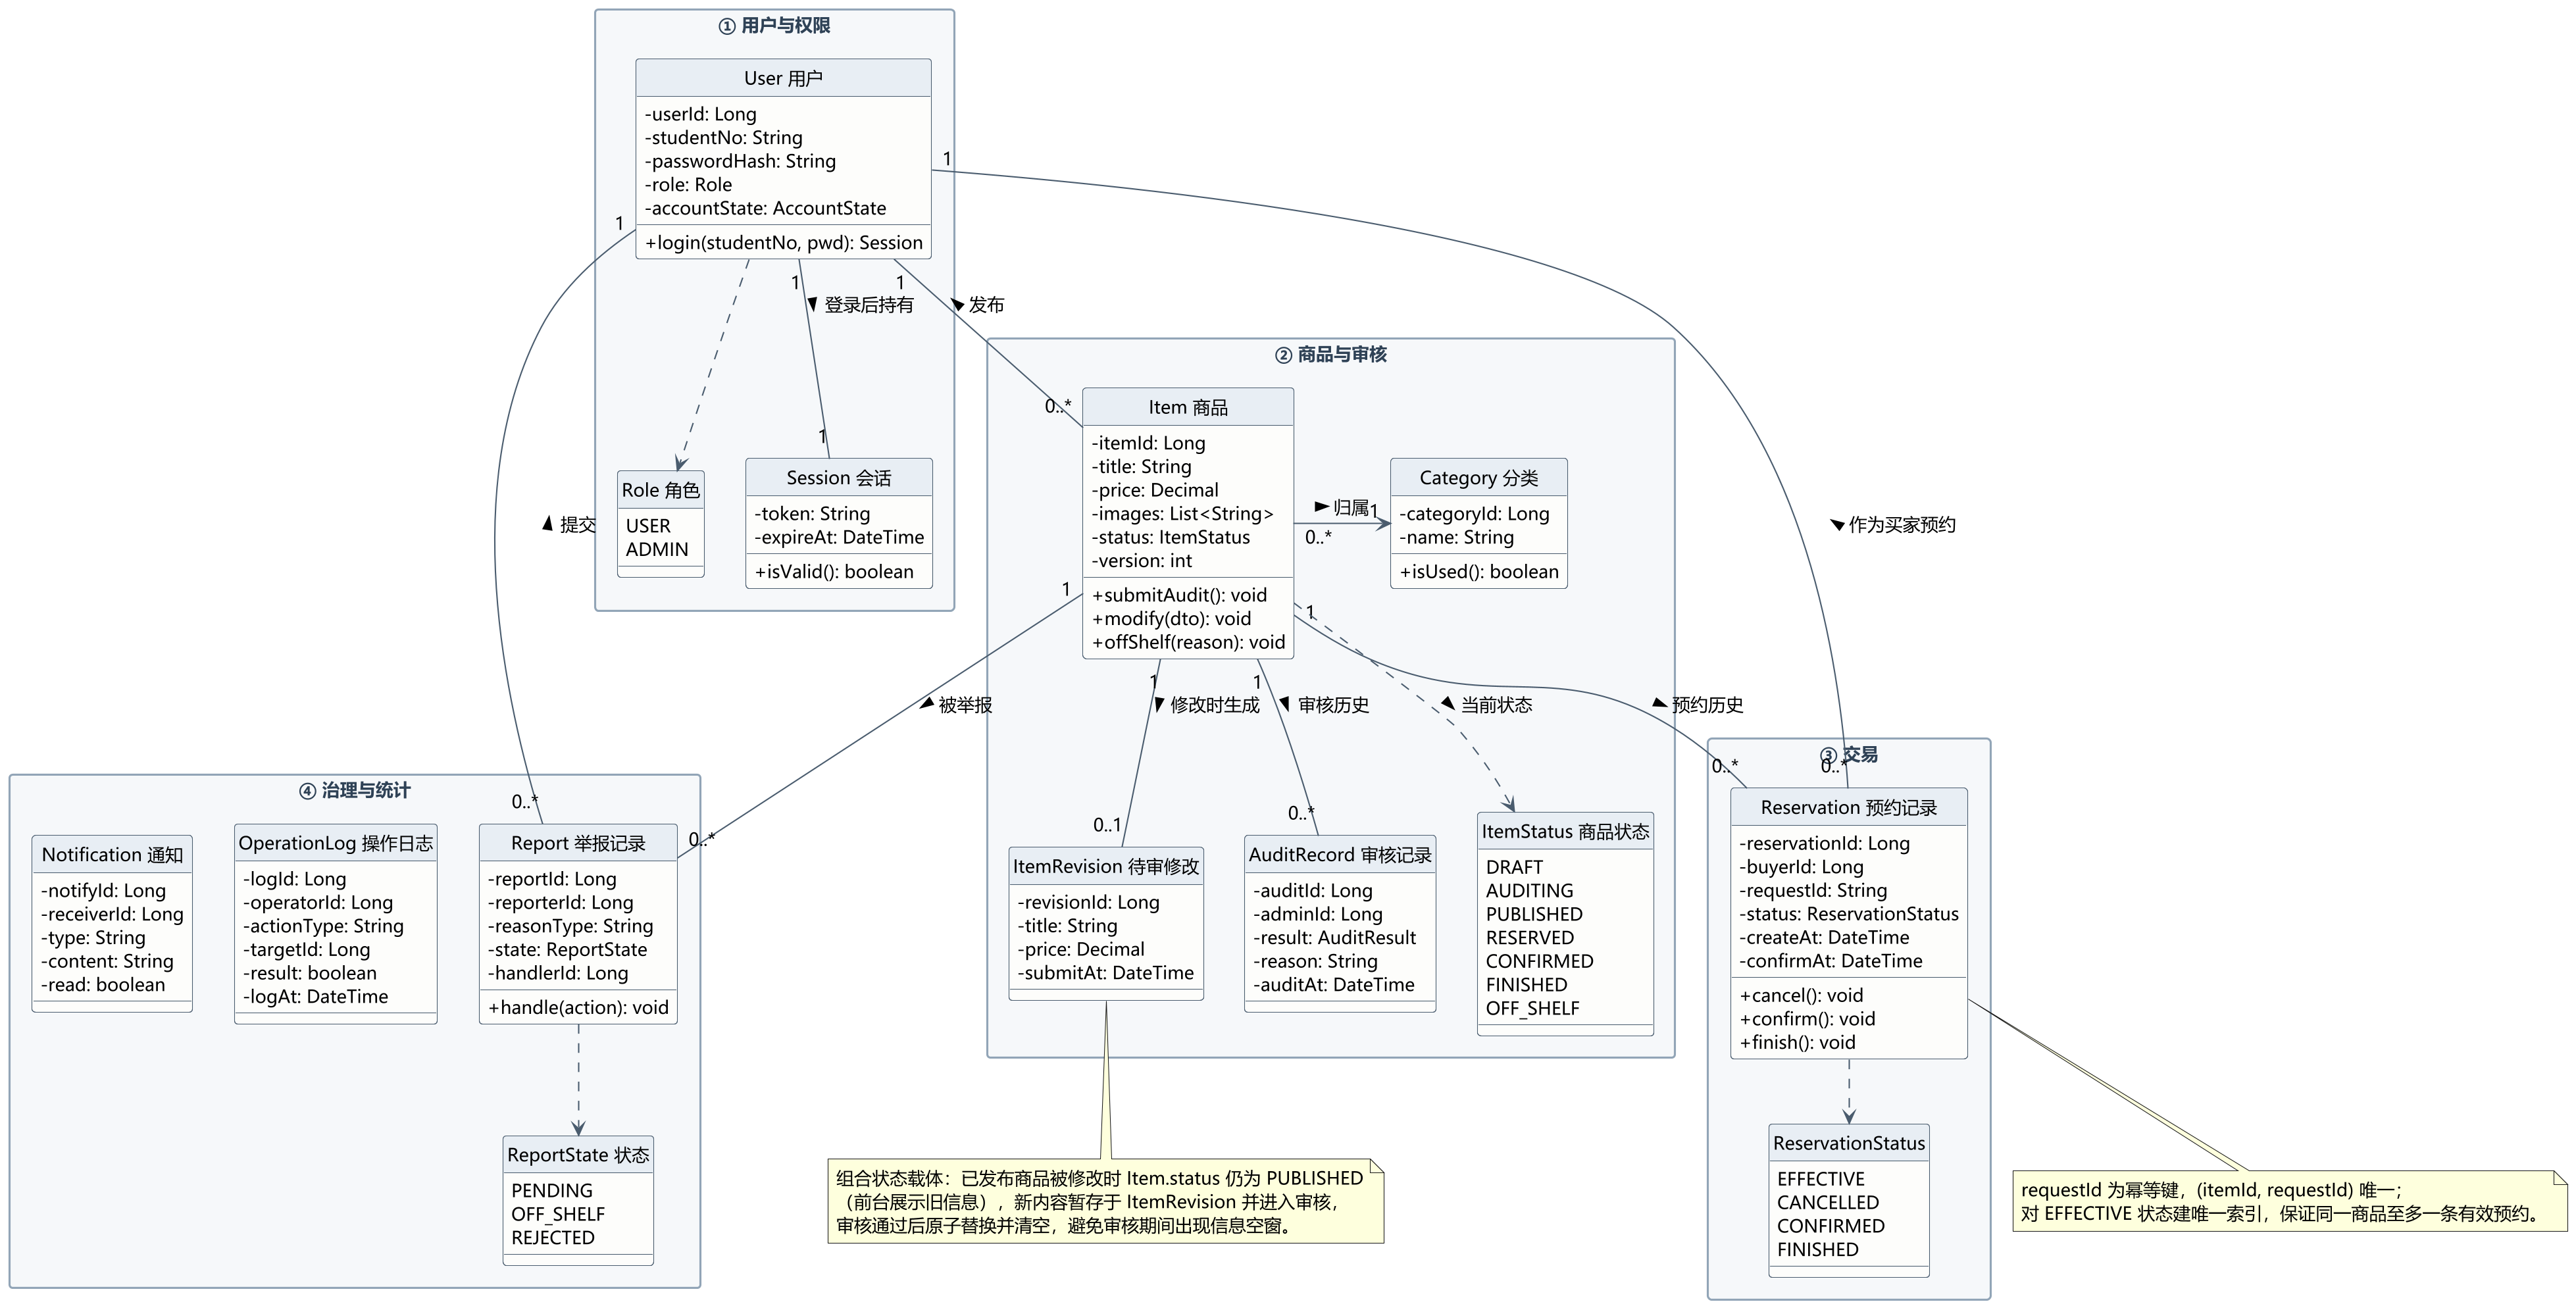
\includegraphics[width=0.99\textwidth]{uml1.png}
\par\vspace{2pt}
\captionof{figure}{校园二手交易系统类图}\label{fig:uml1}
\end{minipage}
\end{center}

类图按用户与权限、商品与审核、交易、治理与统计四个包组织，共 14 个类与枚举。三个关键设计：

\begin{enumerate}[leftmargin=2em,itemsep=1pt]
  \item \textbf{Item 与 ItemRevision 是组合关系}。已发布商品被修改时 Item.status 仍为 PUBLISHED（前台展示旧信息），新内容暂存 ItemRevision 等待审核，通过后原子替换。这是 REQ-017 组合状态在结构上的落点，也解释了“审核期间仍可预约”。
  \item \textbf{实体只暴露状态流转方法}。Item 只有 submitAudit()、modify()、offShelf()，没有 setStatus()，任何状态变更都必须经过校验，从结构上堵住绕过规则改状态。
  \item \textbf{Reservation 携带幂等键 requestId}。商品与预约是一对多，但有效预约唯一；多重性写在连线上会误导实现，因此用注释说明：数据库对 (item\_id, request\_id) 与“状态为 EFFECTIVE 时取 item\_id 的生成列”各建唯一索引，前者保证重复提交不重复创建，后者保证同一商品至多一条有效预约。
\end{enumerate}

\clearpage
\subsection{结构性图（二）：组件图}

\begin{center}
\begin{minipage}{\textwidth}\centering
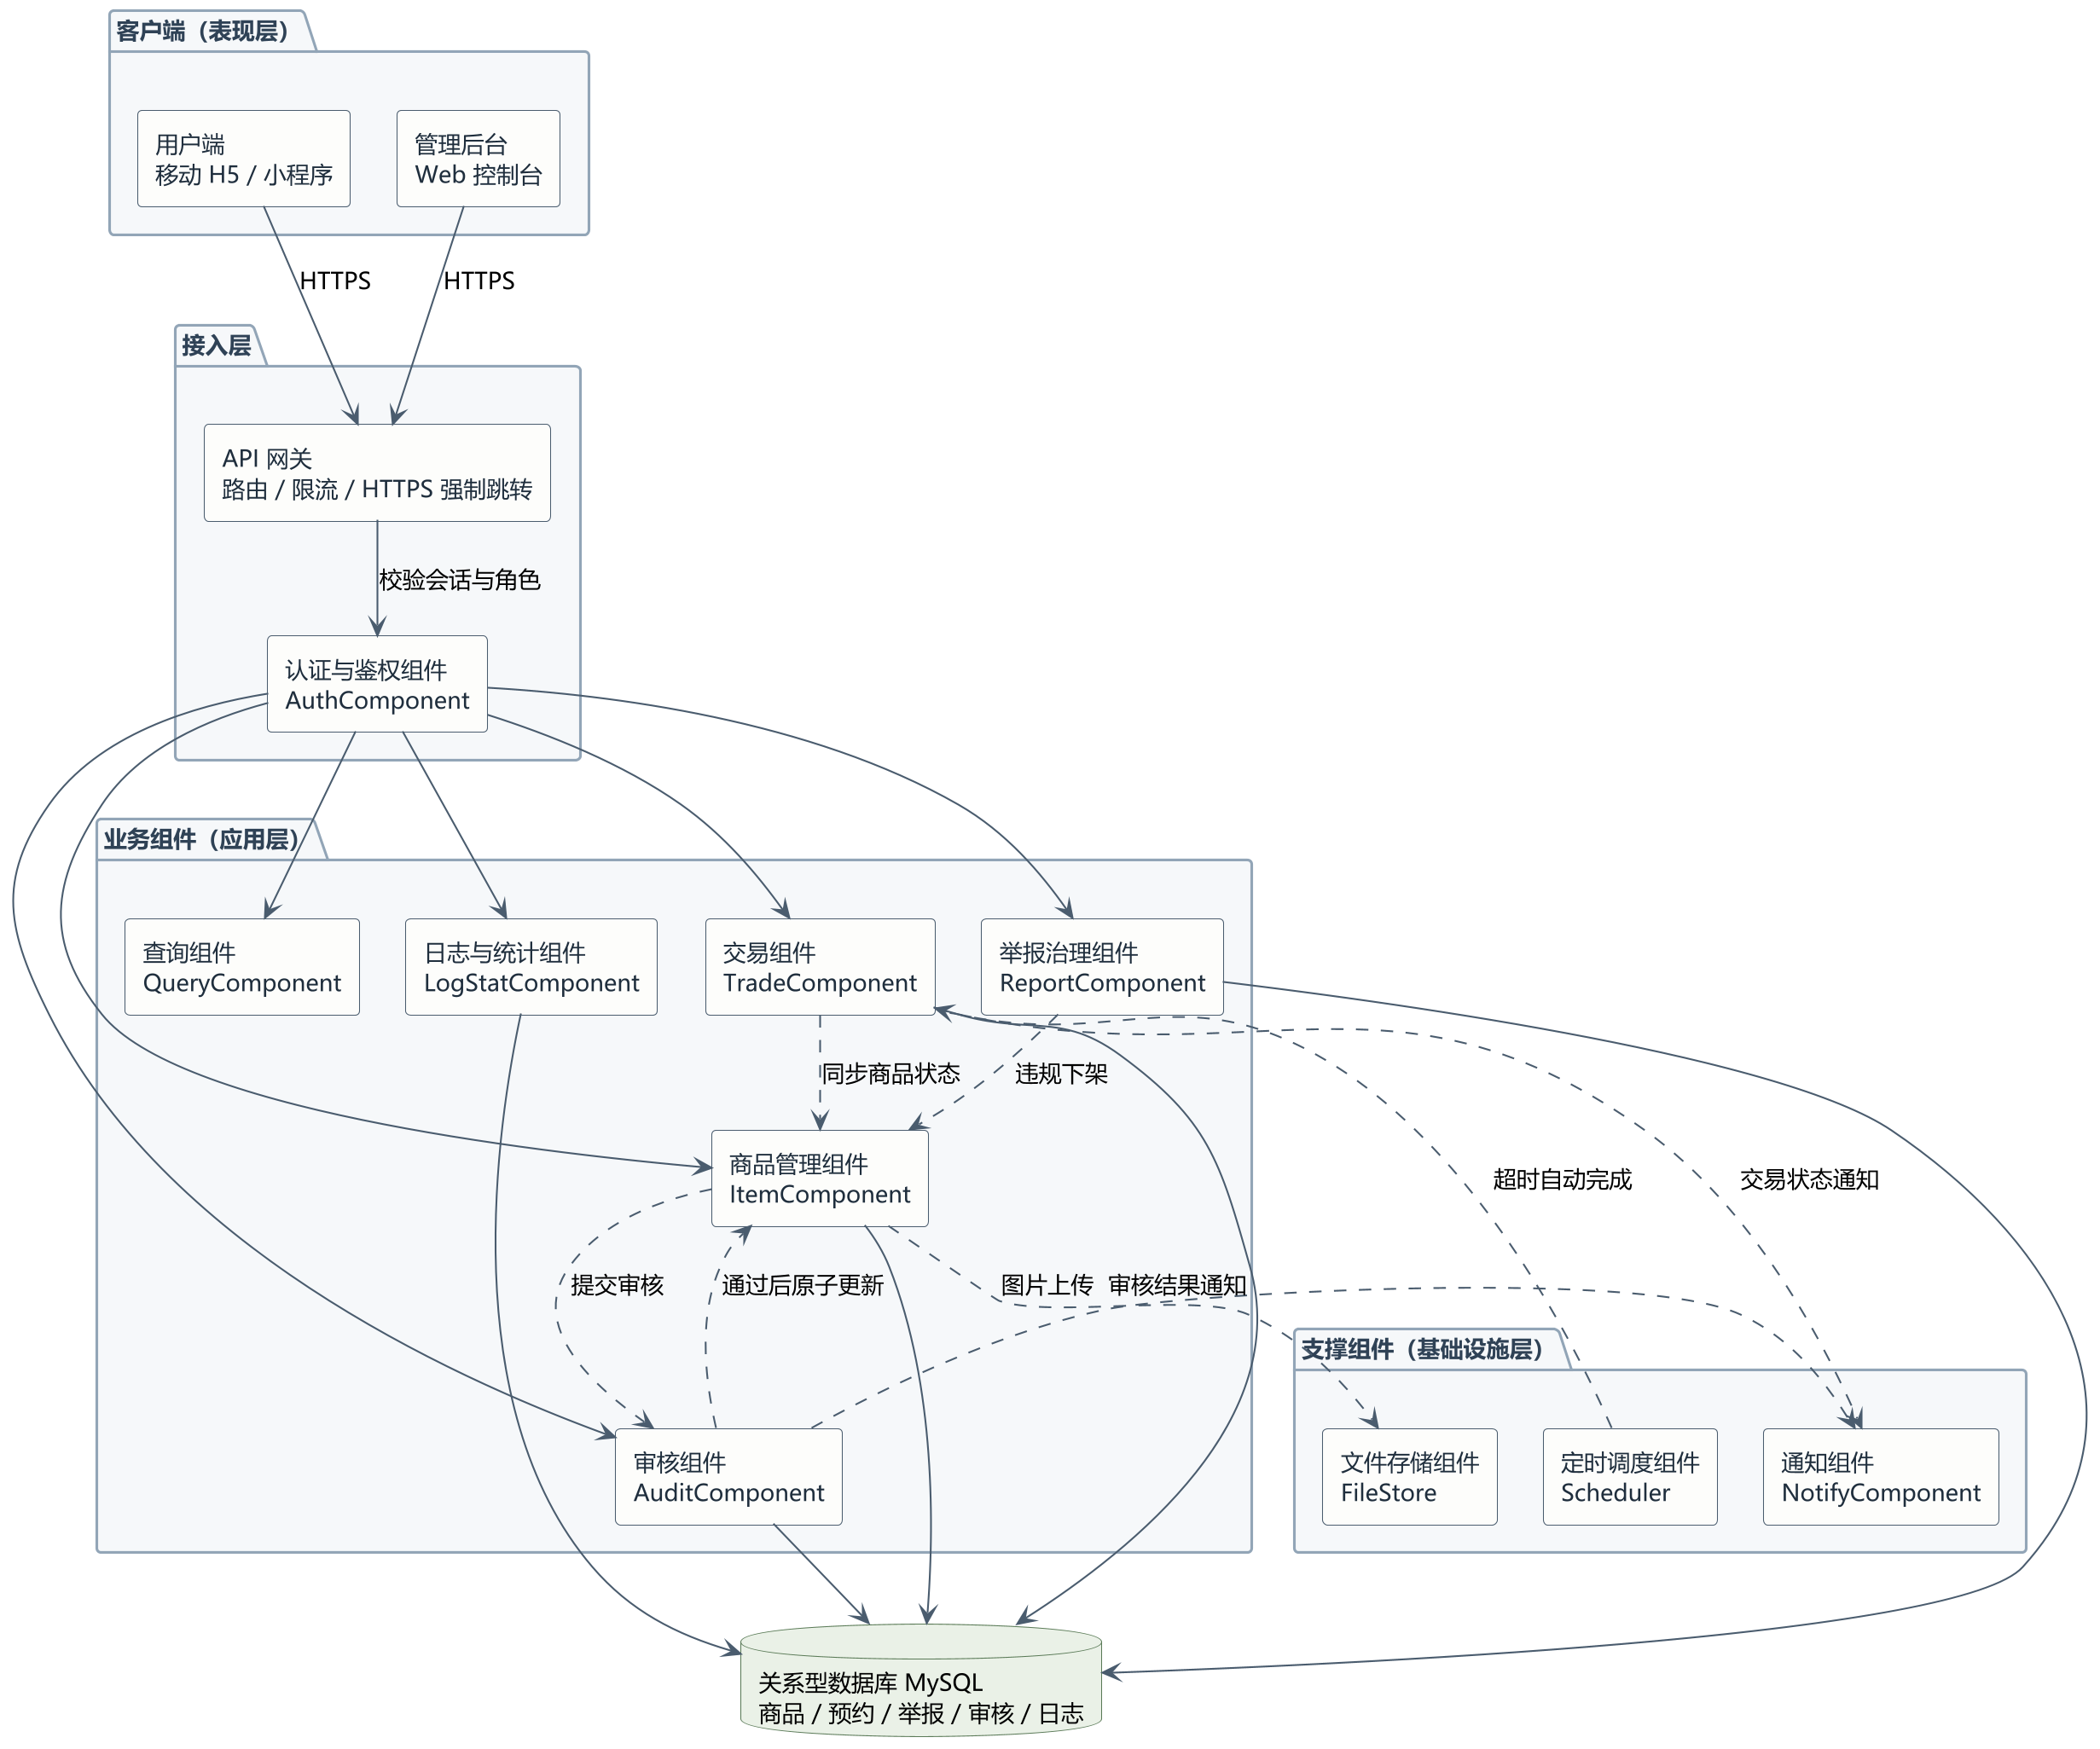
\includegraphics[width=0.88\textwidth]{uml2.png}
\par\vspace{2pt}
\captionof{figure}{校园二手交易系统组件图}\label{fig:uml2}
\end{minipage}
\end{center}

组件图把系统切成客户端、接入层、业务组件、支撑组件四层。客户端只通过 HTTPS 访问 API 网关，网关负责路由、限流与强制跳转 HTTPS（REQ-012），鉴权组件统一校验会话与角色后才分发到业务组件；支撑组件提供通知、定时调度与文件存储，其中定时调度是 REQ-015 超时自动完成的唯一入口。

这样分层的原因是需求中存在大量“状态同步”：预约、审核、举报下架都要改商品状态。如果每个组件都能直接写商品表，一致性只能靠人工保证；组件图用“交易组件 $\rightarrow$ 商品管理组件：同步商品状态”这条依赖说明，状态只有商品组件能写，其他组件只能请求它写。这既是模块边界，也是后续拆分部署的依据。

\clearpage
\subsection{行为性图（一）：用例图}

\begin{center}
\begin{minipage}{\textwidth}\centering
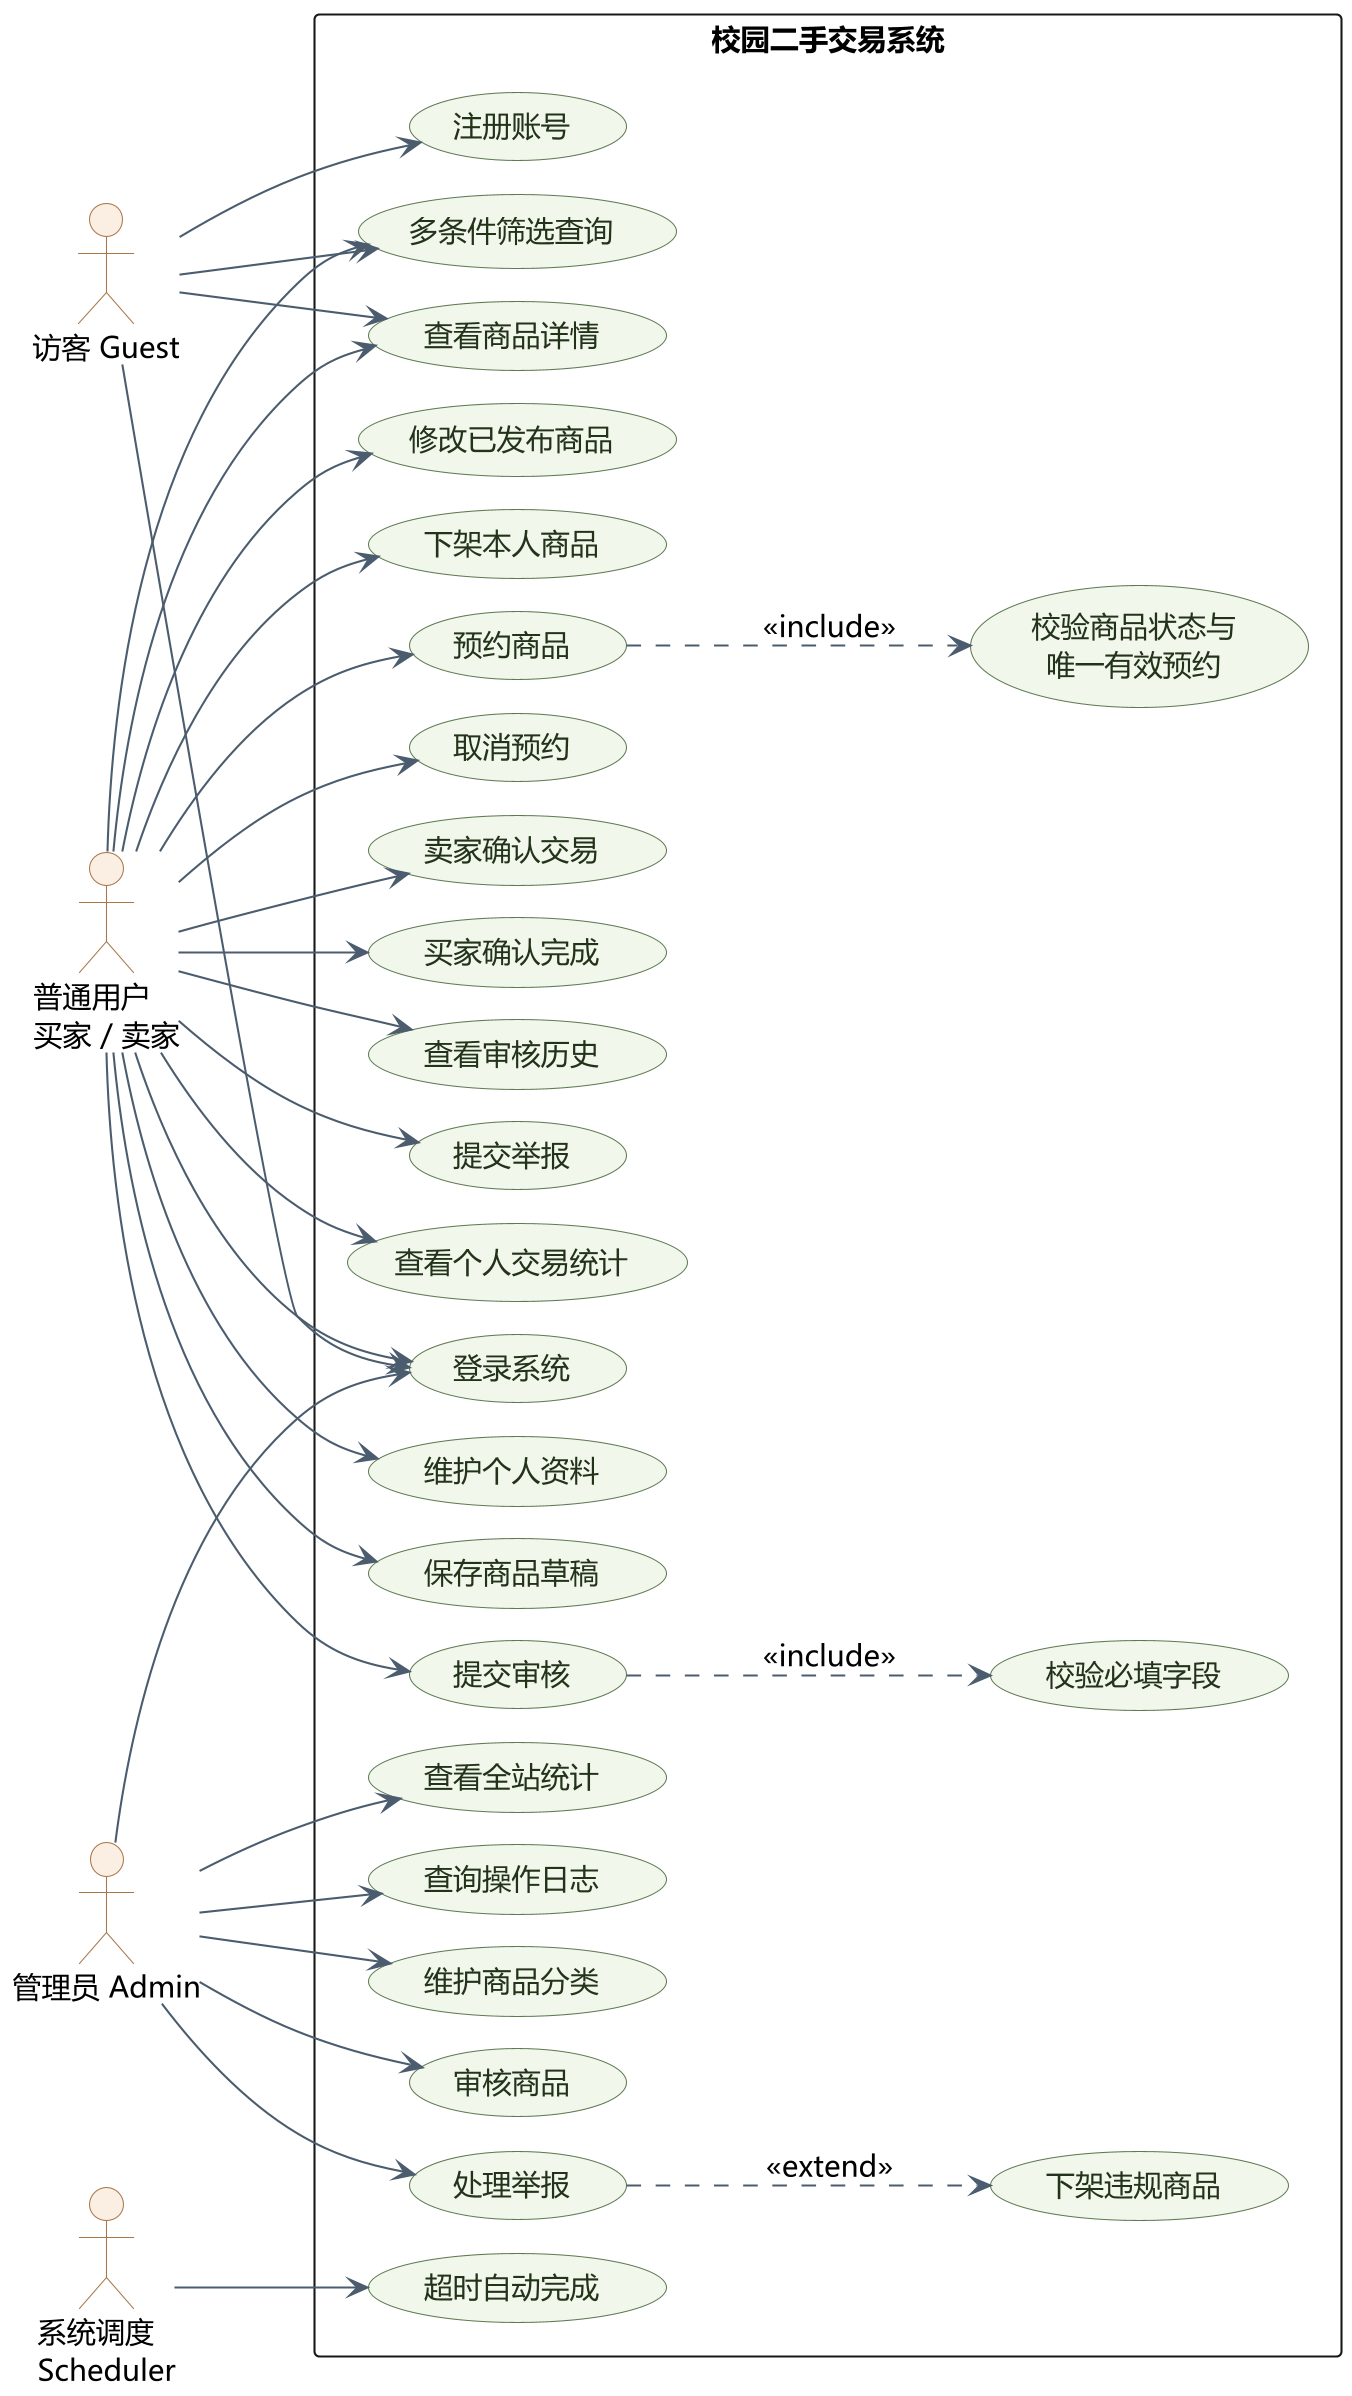
\includegraphics[width=0.54\textwidth]{uml3.png}
\par\vspace{2pt}
\captionof{figure}{校园二手交易系统用例图}\label{fig:uml3}
\end{minipage}
\end{center}

用例图定义四类参与者与 25 个用例。访客可注册、登录、筛选查询与查看详情；普通用户同时是买家和卖家，用例覆盖发布、修改、下架、预约、取消、确认、举报与本人统计；管理员负责审核、举报处置、分类维护、全站统计与日志；系统调度不是人，唯一用例是超时自动完成。

图中标注两个包含关系与一个扩展关系：提交审核包含校验必填字段；预约商品包含校验商品状态与唯一有效预约（并发、重复提交、旧页面、本人商品四个异常都在此判定）；处理举报扩展出下架违规商品。用例图的作用是把 REQ-016 的权限边界画清楚——管理员的用例没有一条连到普通用户，普通用户的用例也没有连到审核与全站统计。

\clearpage
\subsection{行为性图（二）：活动图}

\begin{center}
\begin{minipage}{\textwidth}\centering
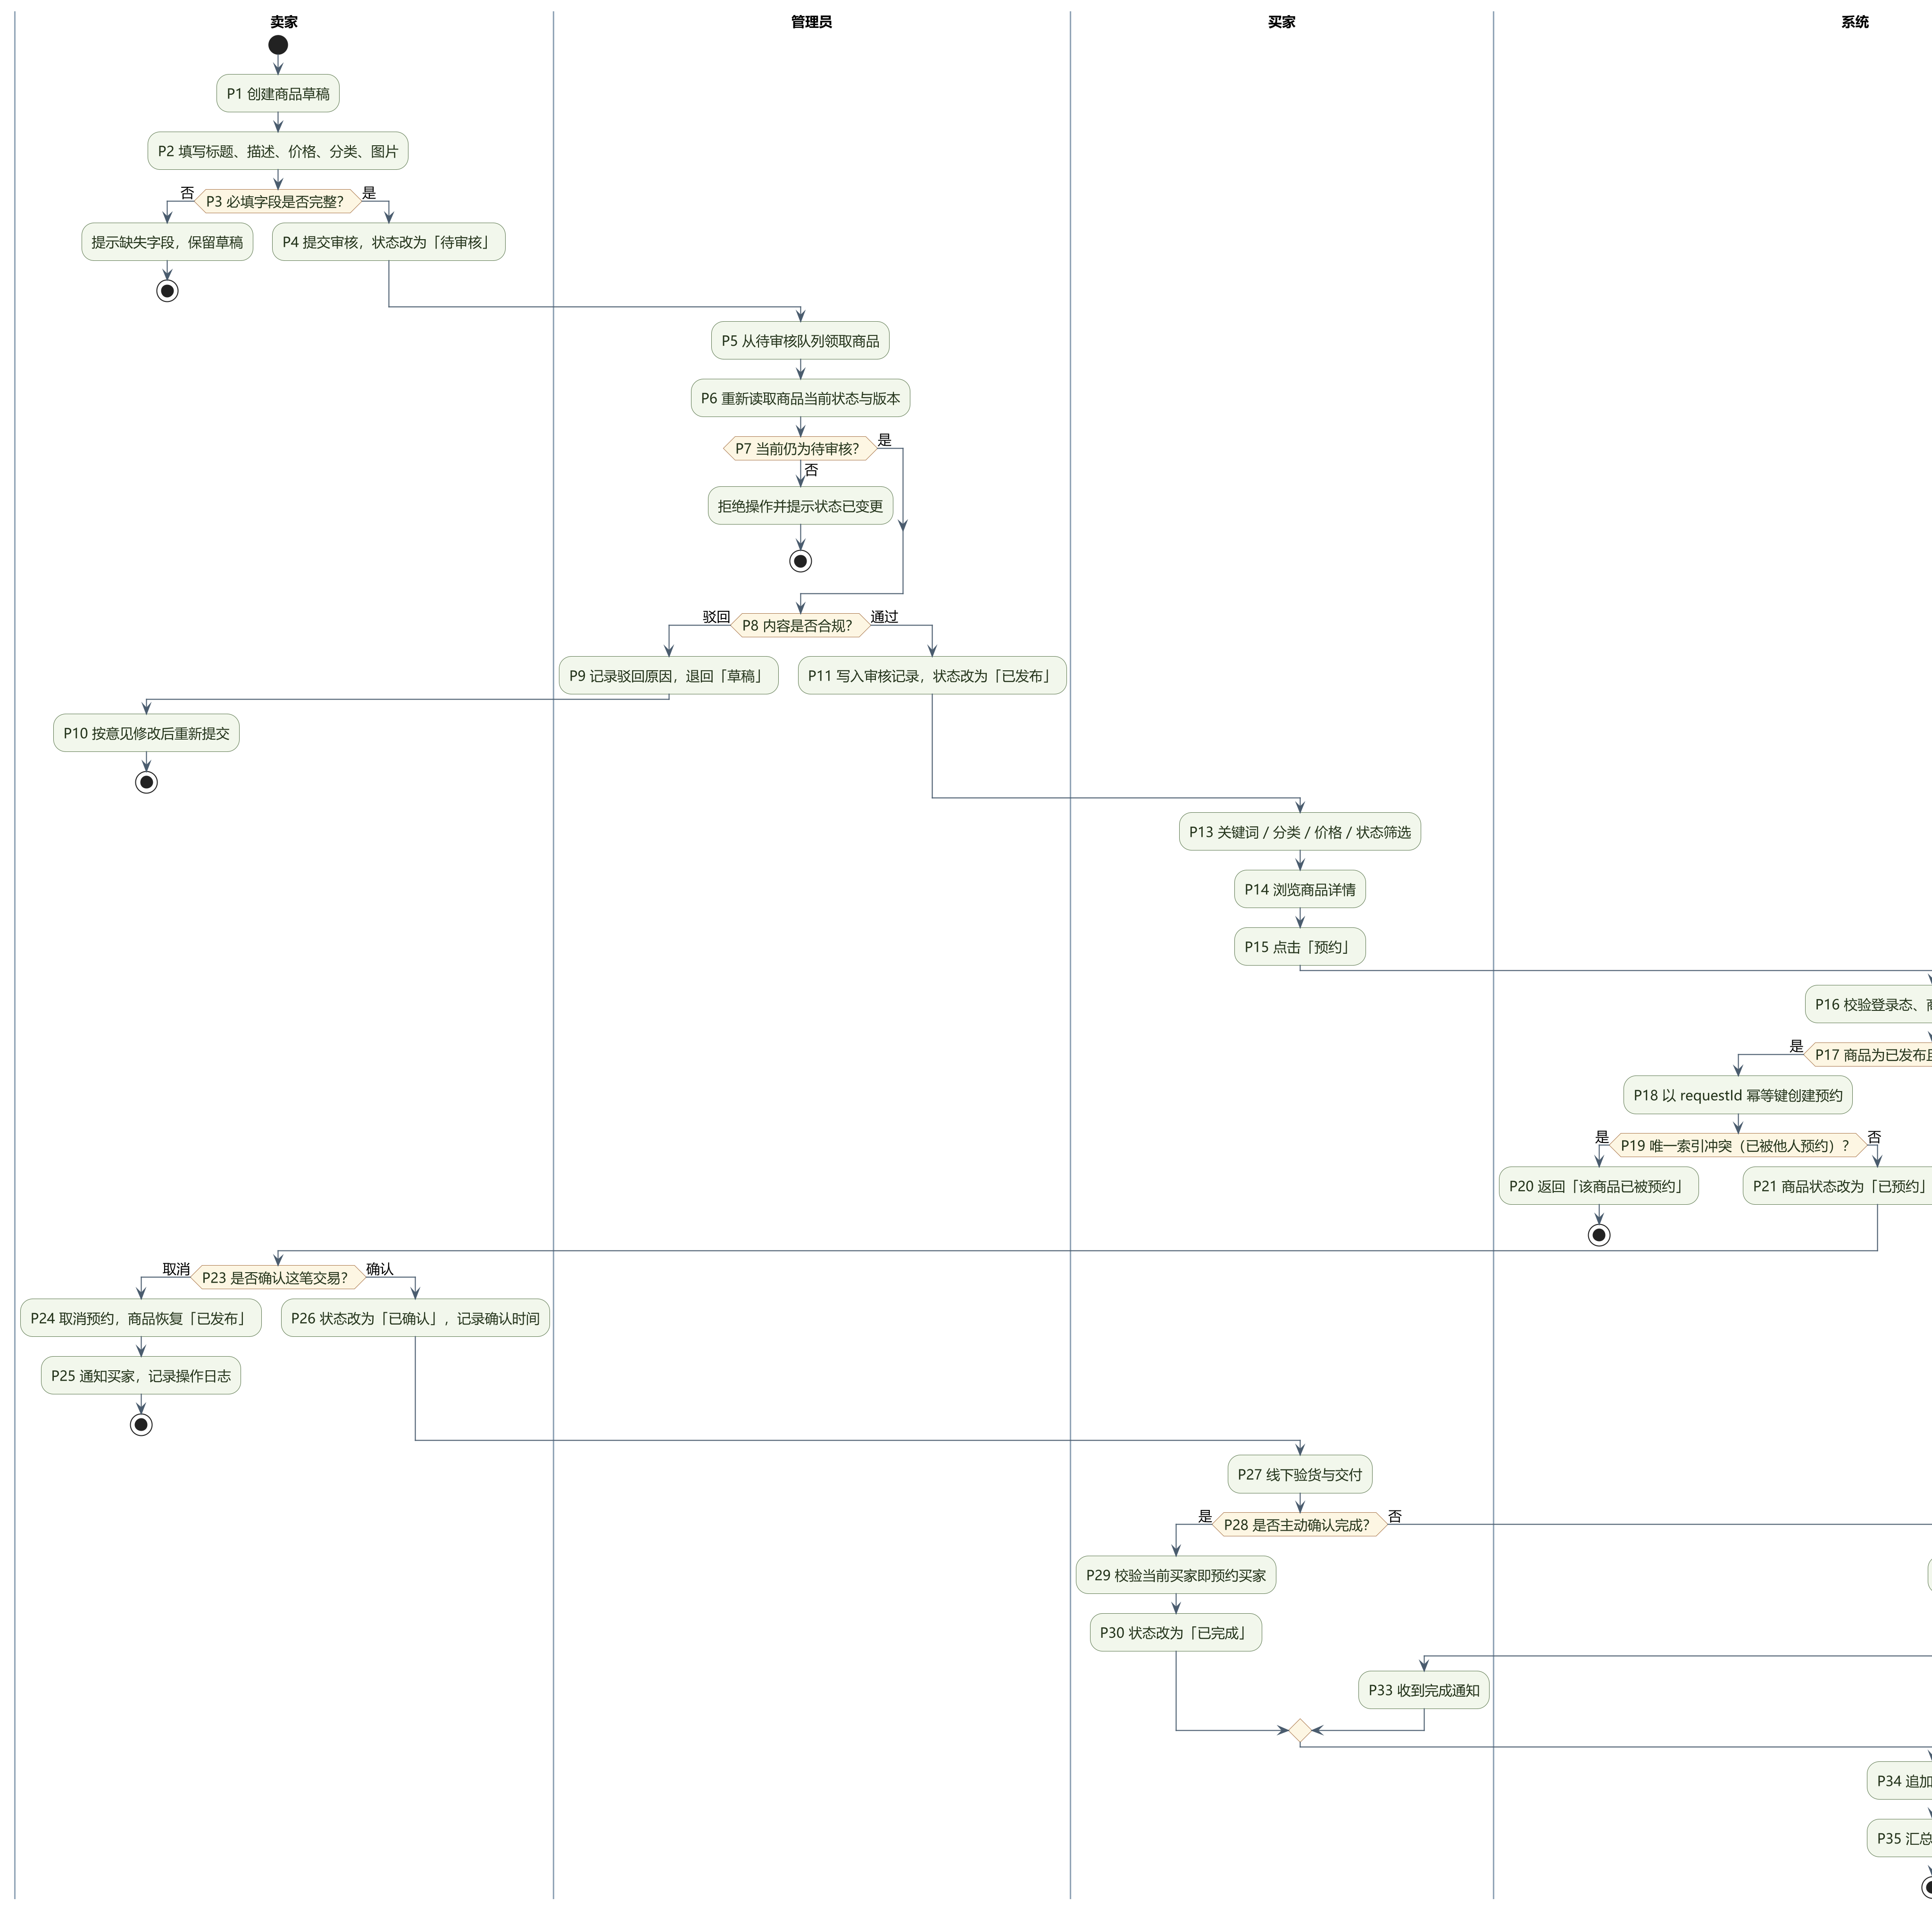
\includegraphics[width=0.96\textwidth]{uml4.png}
\par\vspace{2pt}
\captionof{figure}{商品从发布到完成的主流程活动图（P1--P35）}\label{fig:uml4}
\end{minipage}
\end{center}

活动图用卖家、管理员、买家、系统四条泳道展开完整的交易生命周期，动作编号 P1--P35 便于引用。三个分支直接对应实验一的异常处理：\textbf{P3} 必填字段不完整则保留草稿并终止；\textbf{P7} 管理员领取商品后必须重新读取状态，否则拒绝操作（REQ-003 并发冲突）；\textbf{P17 / P19} 预约的两道闸门，先判“已发布且非本人商品”，再靠唯一索引判并发，失败是显式终止路径而不是异常。

把“系统”单列一条泳道，是因为自动完成容易被误认为由用户触发，从而在实现时漏掉定时任务；P31/P32 放在系统泳道，可直接对应组件图中的定时调度组件。

\clearpage
\subsection{行为性图（三）：状态图}

\begin{center}
\begin{minipage}{\textwidth}\centering
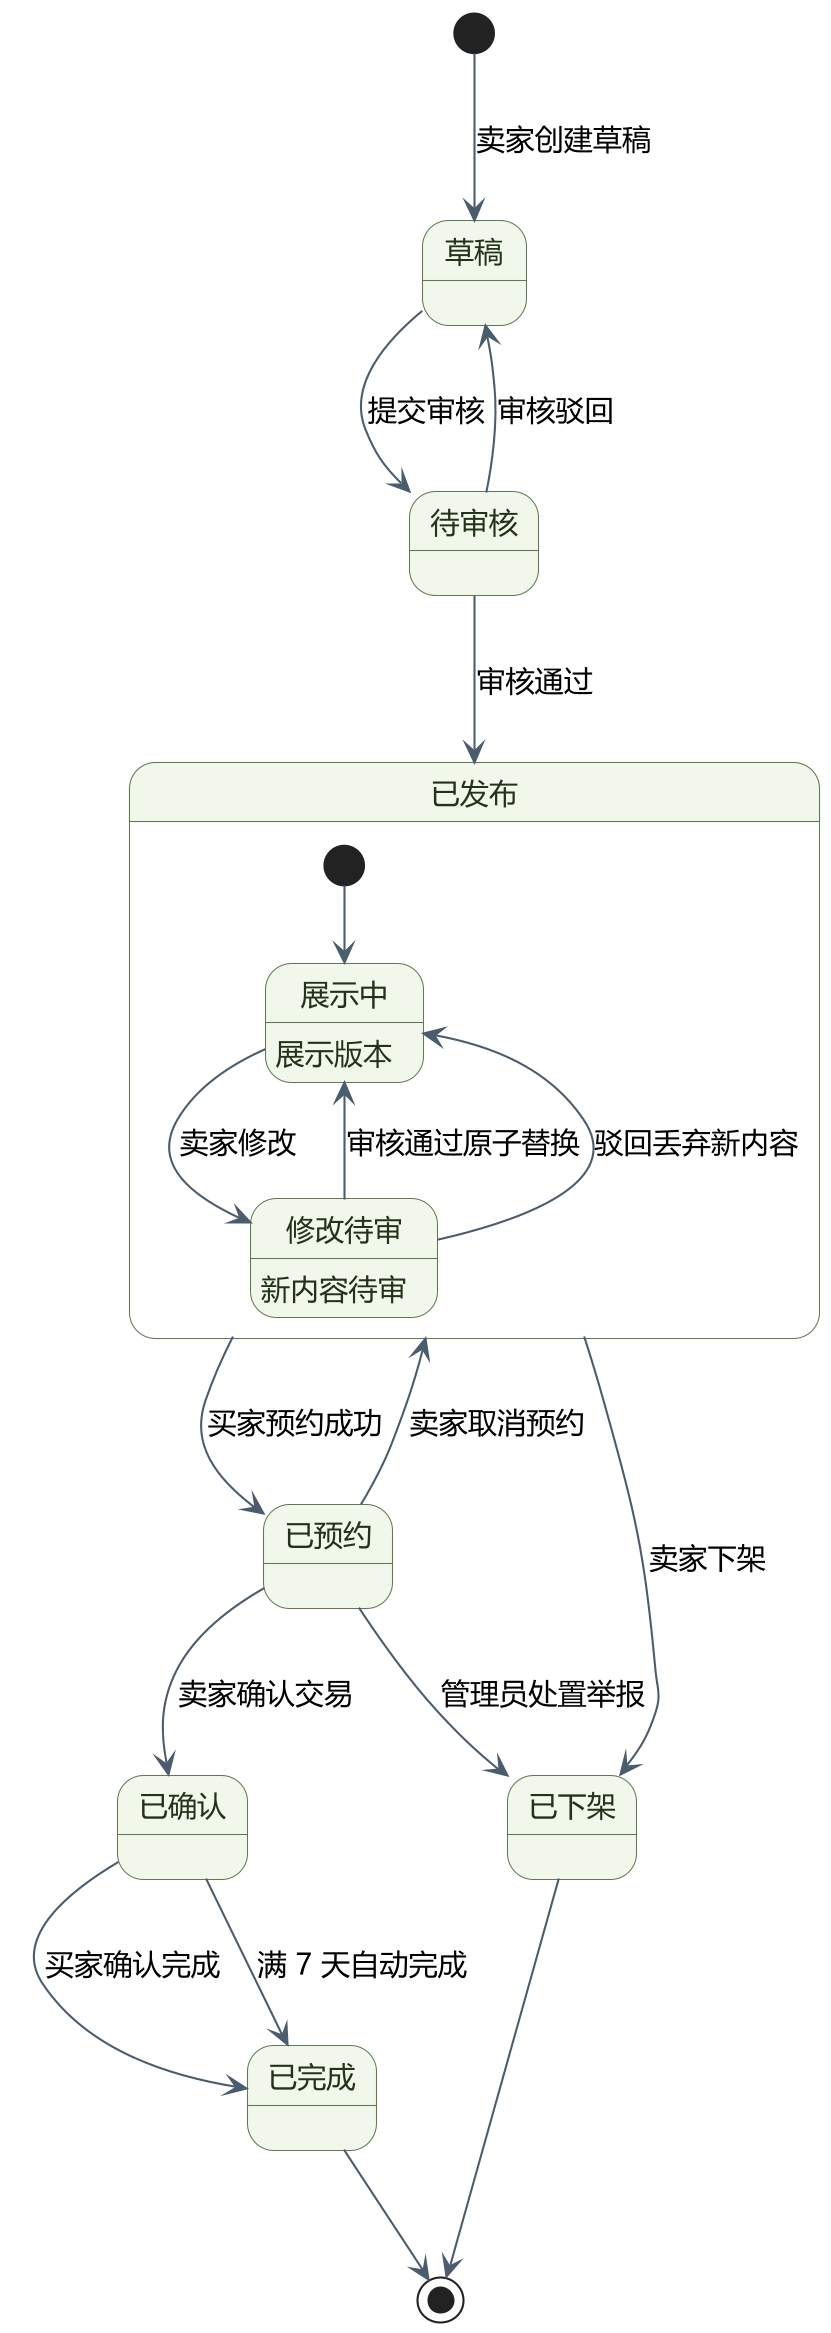
\includegraphics[width=0.34\textwidth]{uml5.png}
\par\vspace{2pt}
\captionof{figure}{商品状态机（含“已发布”组合状态）}\label{fig:uml5}
\end{minipage}
\end{center}

状态图把实验一的状态表图形化，并新增组合状态“已发布”，内部含“展示中”与“修改待审”两个子状态。

之所以用组合状态而不是新增第八个状态，是因为一旦新增，“商品是否可被查询到”“是否可被预约”“统计算不算已发布”三处判断都要同时改，驳回后还要记住原状态。用组合状态后对外可见状态始终是“已发布”，待审内容只是附属对象，通过时原子替换、驳回时直接丢弃。

图中刻意没有画“已完成 $\rightarrow$ 已预约”“已下架 $\rightarrow$ 已发布”，实验一明确禁止这些转换，用“不画”表达禁止比画一条打叉的线更清晰：从已完成与已下架只有指向终态的转移。

\clearpage
\subsection{交互性图：时序图}

\begin{center}
\begin{minipage}{\textwidth}\centering
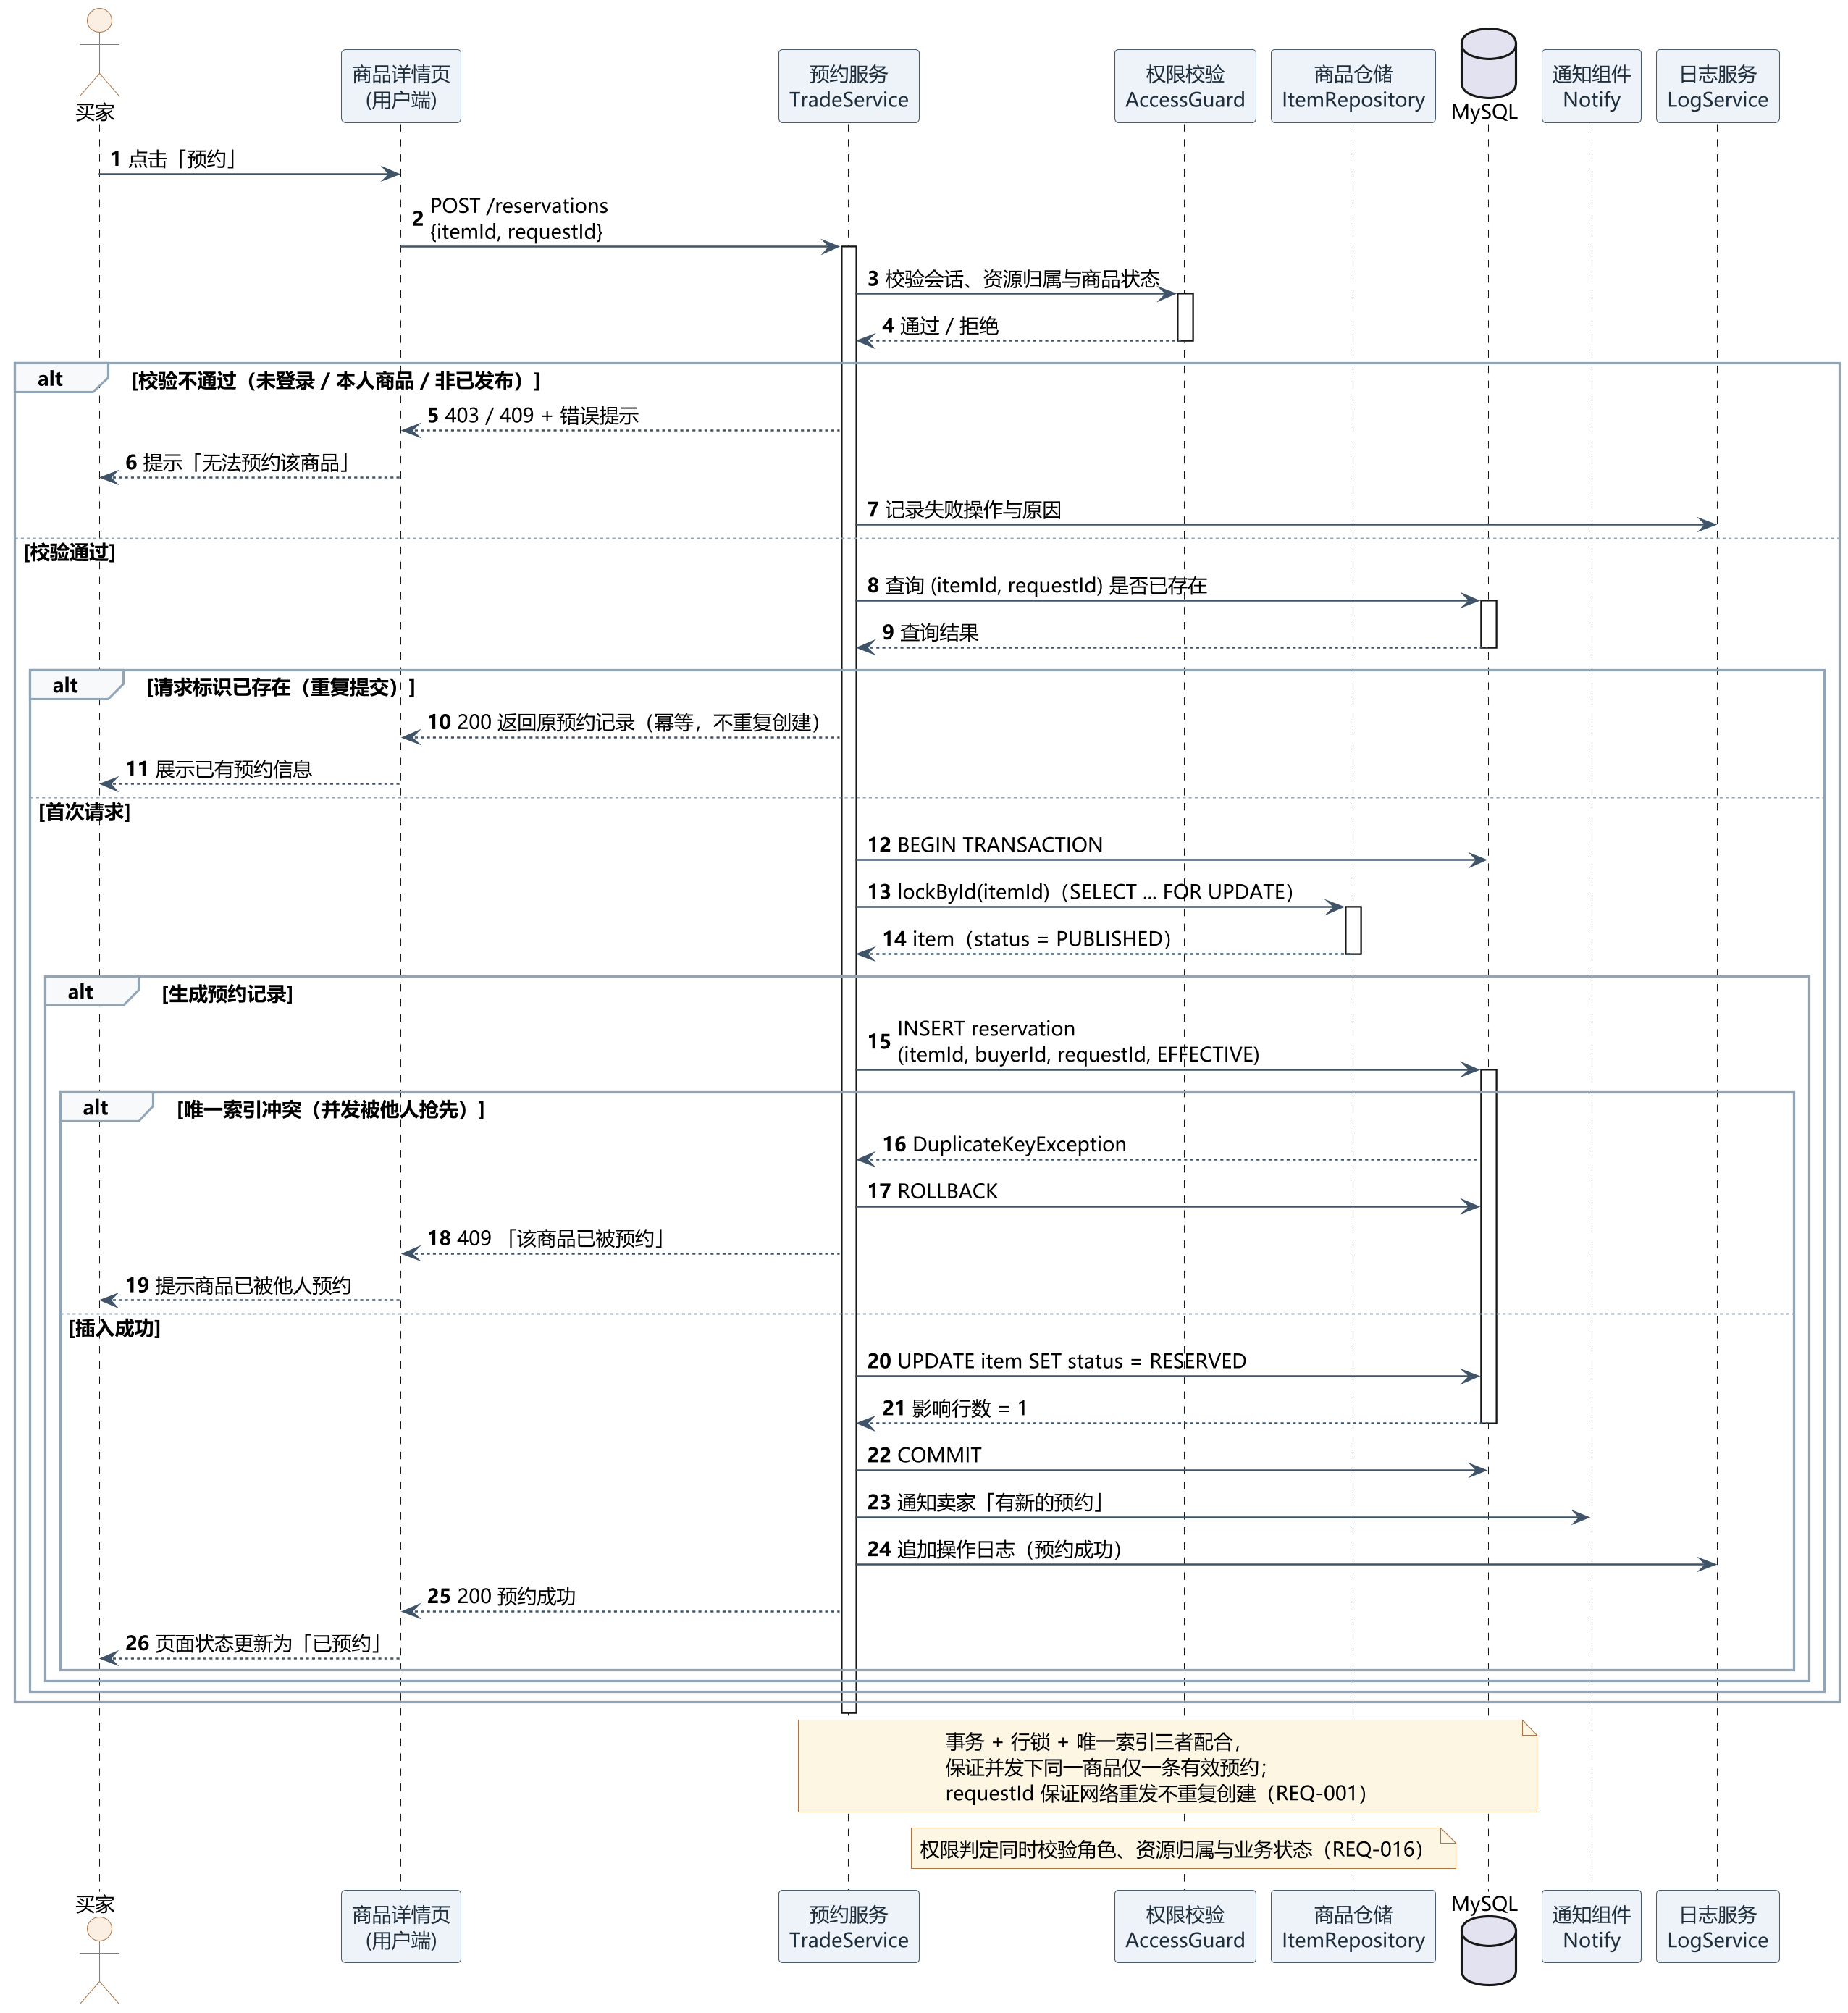
\includegraphics[width=0.84\textwidth]{uml6.png}
\par\vspace{2pt}
\captionof{figure}{商品预约时序图（含幂等与并发控制）}\label{fig:uml6}
\end{minipage}
\end{center}

时序图选择全系统最复杂的动作——预约，8 条生命线、26 条消息、三层嵌套分支。

\begin{enumerate}[leftmargin=2em,itemsep=1pt]
  \item \textbf{先鉴权后业务}：同时检查会话、商品归属与商品状态，任一不满足即返回 403/409，失败也要写日志——预约本人商品、旧页面预约已成交商品本身需要留痕。
  \item \textbf{幂等查重前置}：以 (itemId, requestId) 查重，命中直接返回原记录。必须在加锁之前完成，否则重复请求会排队等锁。
  \item \textbf{事务内加锁插入}：开事务后对商品行加锁再插入，唯一索引冲突则回滚返回“已被预约”，成功则更新商品状态后提交。行锁、唯一索引、事务缺一不可：只有唯一索引无法区分“重复提交”与“别人抢先”，只有行锁则重发仍会重复创建。
\end{enumerate}

实验一的两条验收标准在此一一对应：并发只留一条有效记录对应唯一索引冲突分支，重发记录数不增加对应幂等分支。

\clearpage
\section{各功能模块的 UI 界面及功能描述}

界面共 10 个：用户端 6 个（移动端 390$\times$844），管理后台 4 个（桌面端 1280$\times$820）。分两种尺寸是因为使用场景不同——学生在手机上碎片时间浏览与预约，管理员在电脑上批量审核与查日志，把管理功能塞进手机界面会为了适配小屏牺牲表格的对比效率。

设计遵循四条原则：状态可见（处在哪个状态、下一步能做什么一屏看清）、风险前置（不可逆操作前给出规则提示）、一屏一任务、两端一致（绿色可用、橙色注意、红色失败或违规）。主色 \#0E9F6E，价格色 \#F4511E，正文 \#16202B。8 个模块全部有界面承接，M8 公共支撑属于后端能力，以“消息”“图片上传”“超时自动完成提示”的形式出现在其他界面中。界面稿以 HTML/CSS 搭成可交互原型，按 2 倍分辨率导出为图片，10 个界面共用同一套颜色、字号、圆角与间距令牌。

\subsection{用户端界面}

\begin{center}
\begin{minipage}{0.97\textwidth}\centering
\begin{minipage}{0.41\linewidth}\centering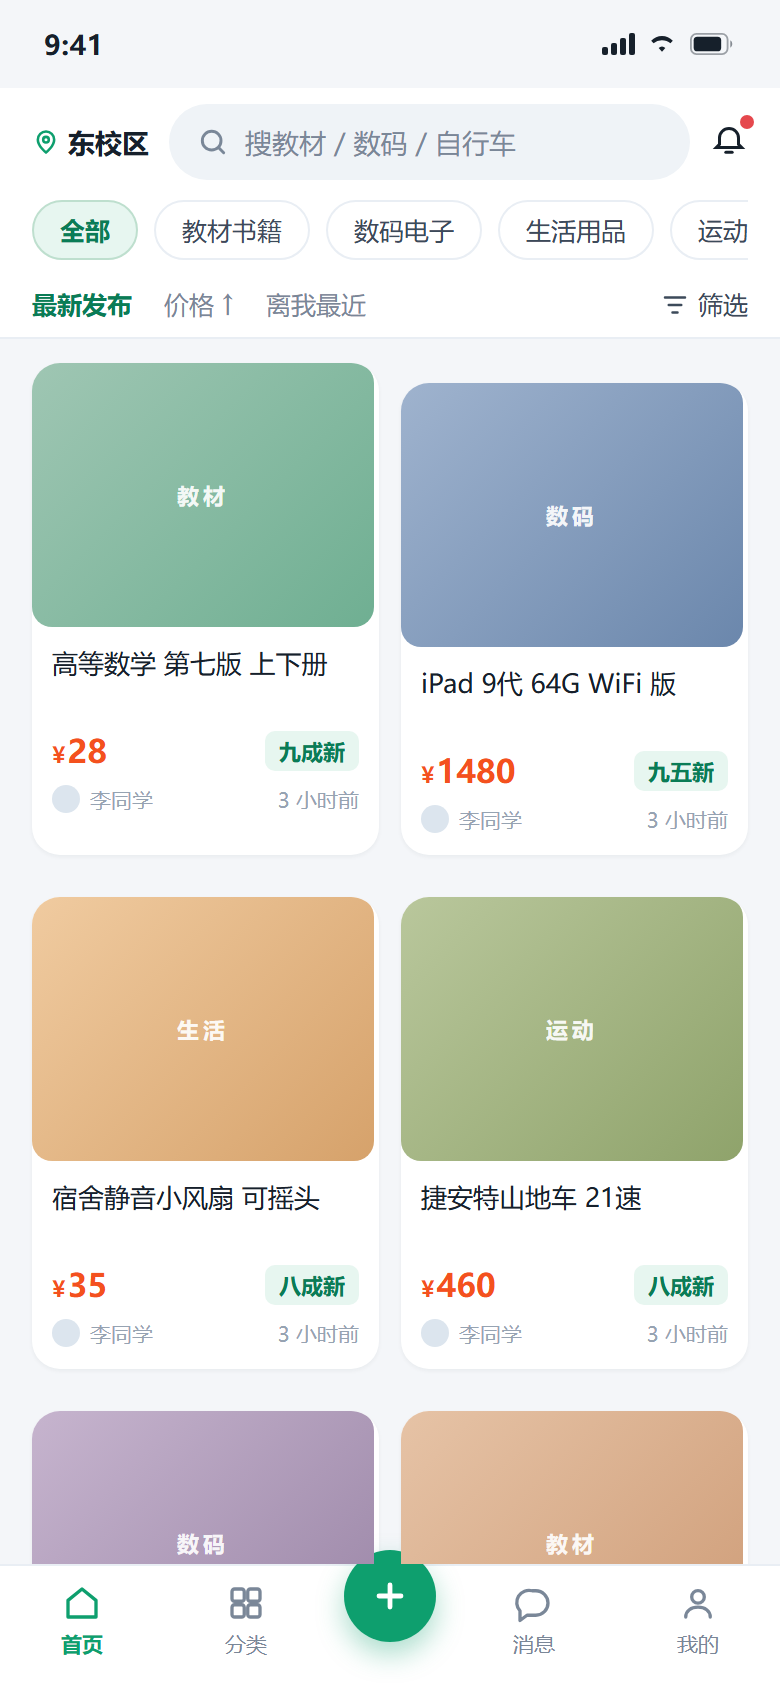
\includegraphics[width=\linewidth]{ui1.png}\end{minipage}\hfill
\begin{minipage}{0.41\linewidth}\centering
\includegraphics[width=\linewidth]{ui2.png}\end{minipage}
\par\vspace{2pt}
\captionof{figure}{界面 1 首页·商品查询（左）与界面 2 商品详情·预约（右）}\label{fig:ui12}
\end{minipage}
\end{center}

\textbf{界面 1}：顶部为位置、搜索框与消息入口，第二行分类快筛，第三行排序与筛选；商品以双列卡片呈现封面、标题、价格、成色、卖家与时间。公开列表只出现已发布商品，已预约、已确认、已完成、已下架的商品不在此出现（REQ-005）；成色用标签而非文字描述，便于扫视判断。

\textbf{界面 2}：大图区、价格与状态、卖家信息、交易地点与审核状态、商品描述，底部固定“举报 / 联系卖家 / 立即预约”。价格区直接标注“已发布”，用户不必猜商品是否还能预约；底部提示条写明“同一商品只支持一条有效预约”，把 REQ-001 的规则前置到操作之前；商品已被预约时按钮替换为不可点击的“已被预约”。

\begin{center}
\begin{minipage}{0.97\textwidth}\centering
\begin{minipage}{0.41\linewidth}\centering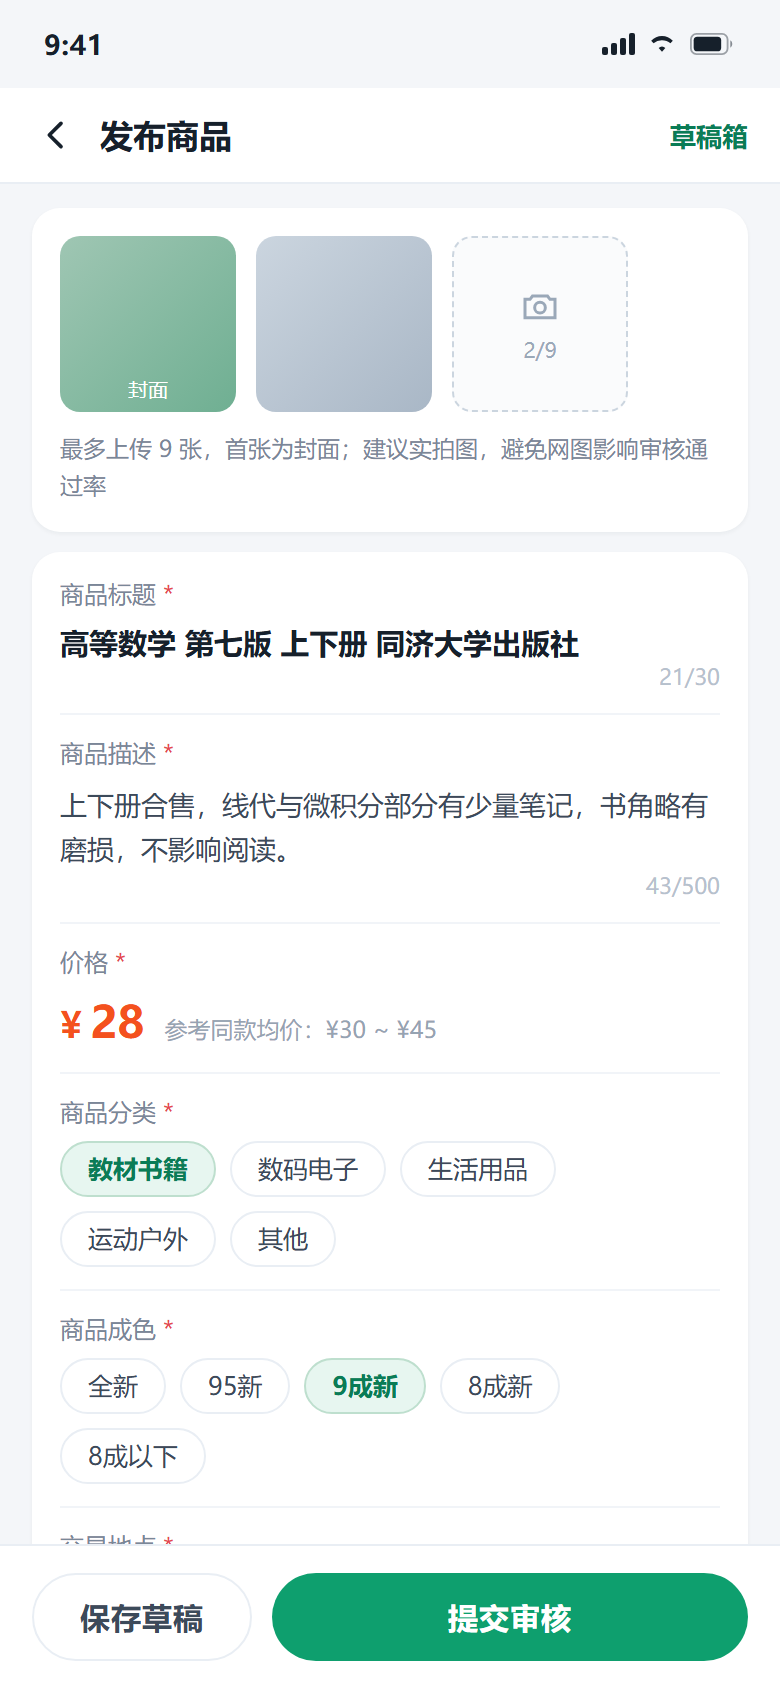
\includegraphics[width=\linewidth]{ui3.png}\end{minipage}\hfill
\begin{minipage}{0.41\linewidth}\centering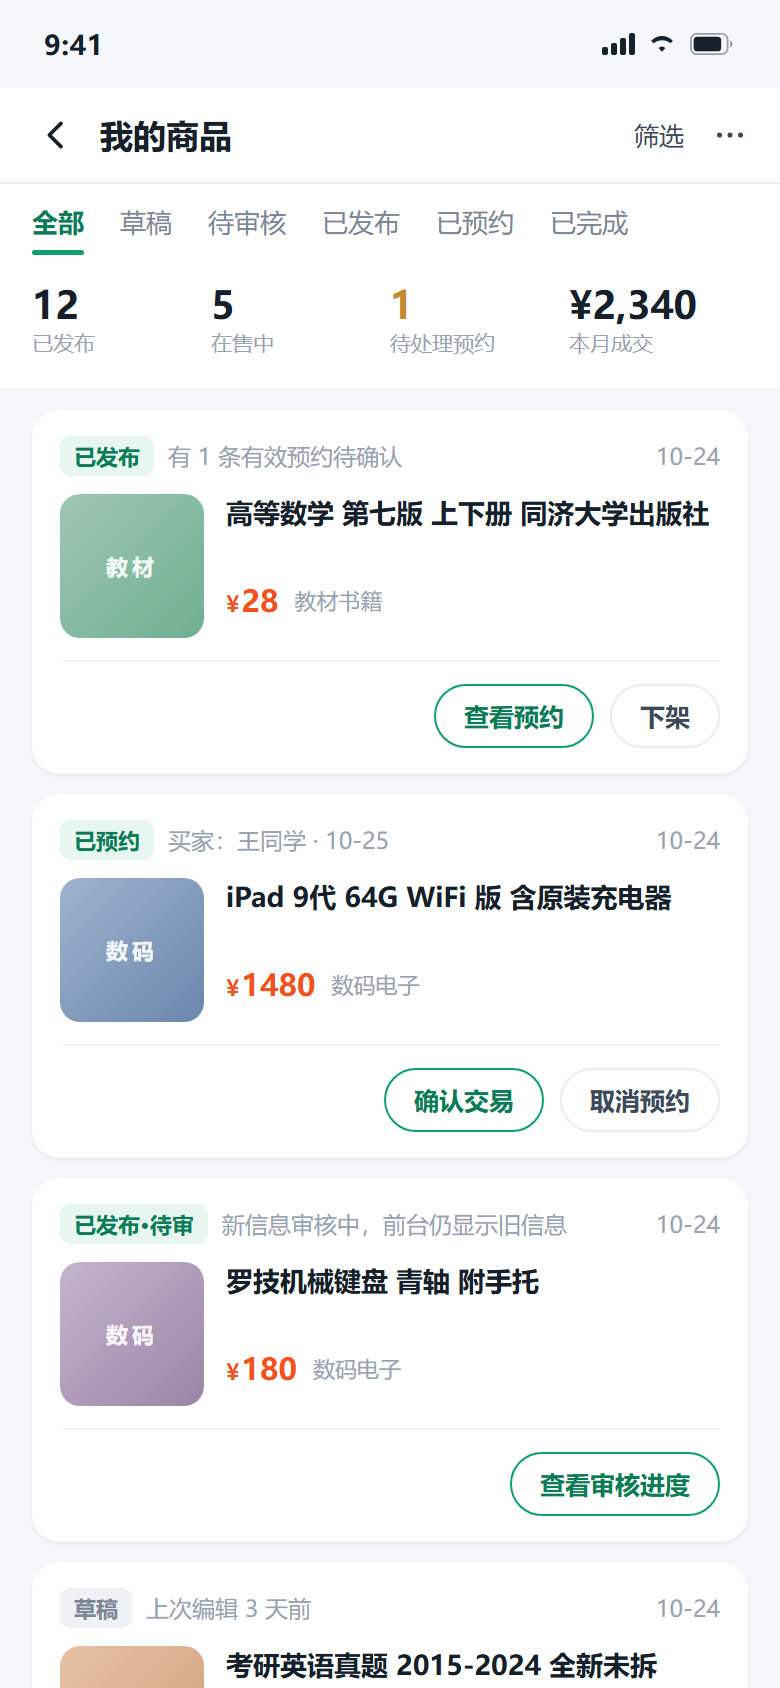
\includegraphics[width=\linewidth]{ui4.png}\end{minipage}
\par\vspace{2pt}
\captionof{figure}{界面 3 发布商品（左）与界面 4 我的商品（右）}\label{fig:ui34}
\end{minipage}
\end{center}

\textbf{界面 3}：九宫格图片上传（首张为封面）、标题、描述、价格、分类、成色、交易地点，必填项用红色星号标注，价格下方给出同款均价。提示条说明“提交后进入审核队列，审核通过前不会出现在公开列表”，把审核流程透明化；底部“保存草稿”与“提交审核”并列，对应 REQ-002 的两种保存方式。

\textbf{界面 4}：顶部按状态分栏，下方四个统计数字，列表项以状态标签开头，右侧只给出当前状态允许的操作。这是“组合状态”唯一能被用户看见的地方——第三个商品显示“已发布·待审”，说明新内容在审核、前台仍展示旧信息（REQ-017）；“确认交易 / 取消预约”只出现在已预约商品上，“下架”只出现在已发布商品上，按钮与状态严格绑定。

\begin{center}
\begin{minipage}{0.97\textwidth}\centering
\begin{minipage}{0.41\linewidth}\centering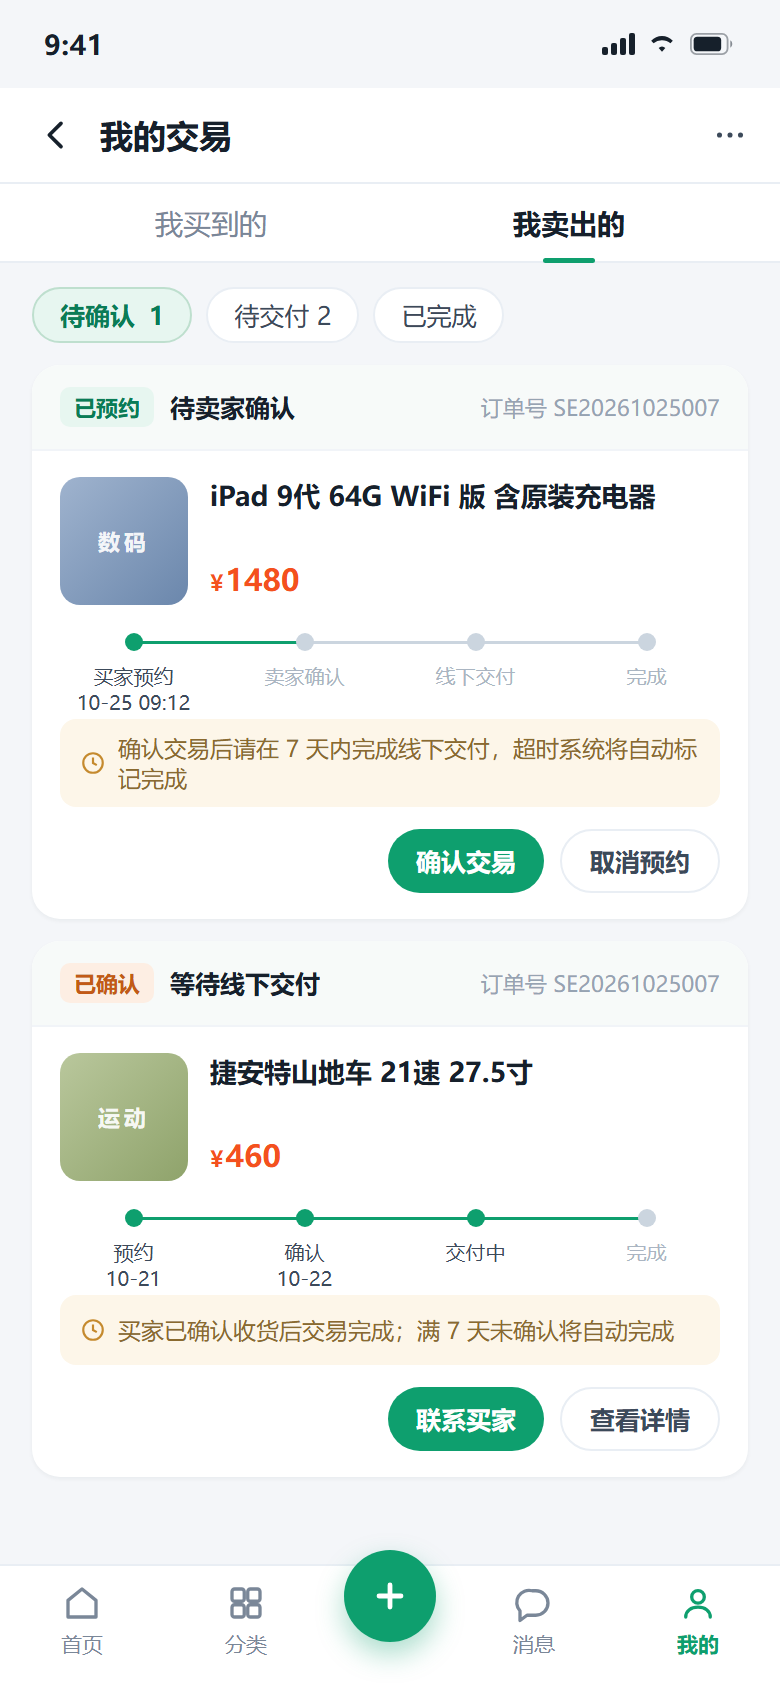
\includegraphics[width=\linewidth]{ui5.png}\end{minipage}\hfill
\begin{minipage}{0.41\linewidth}\centering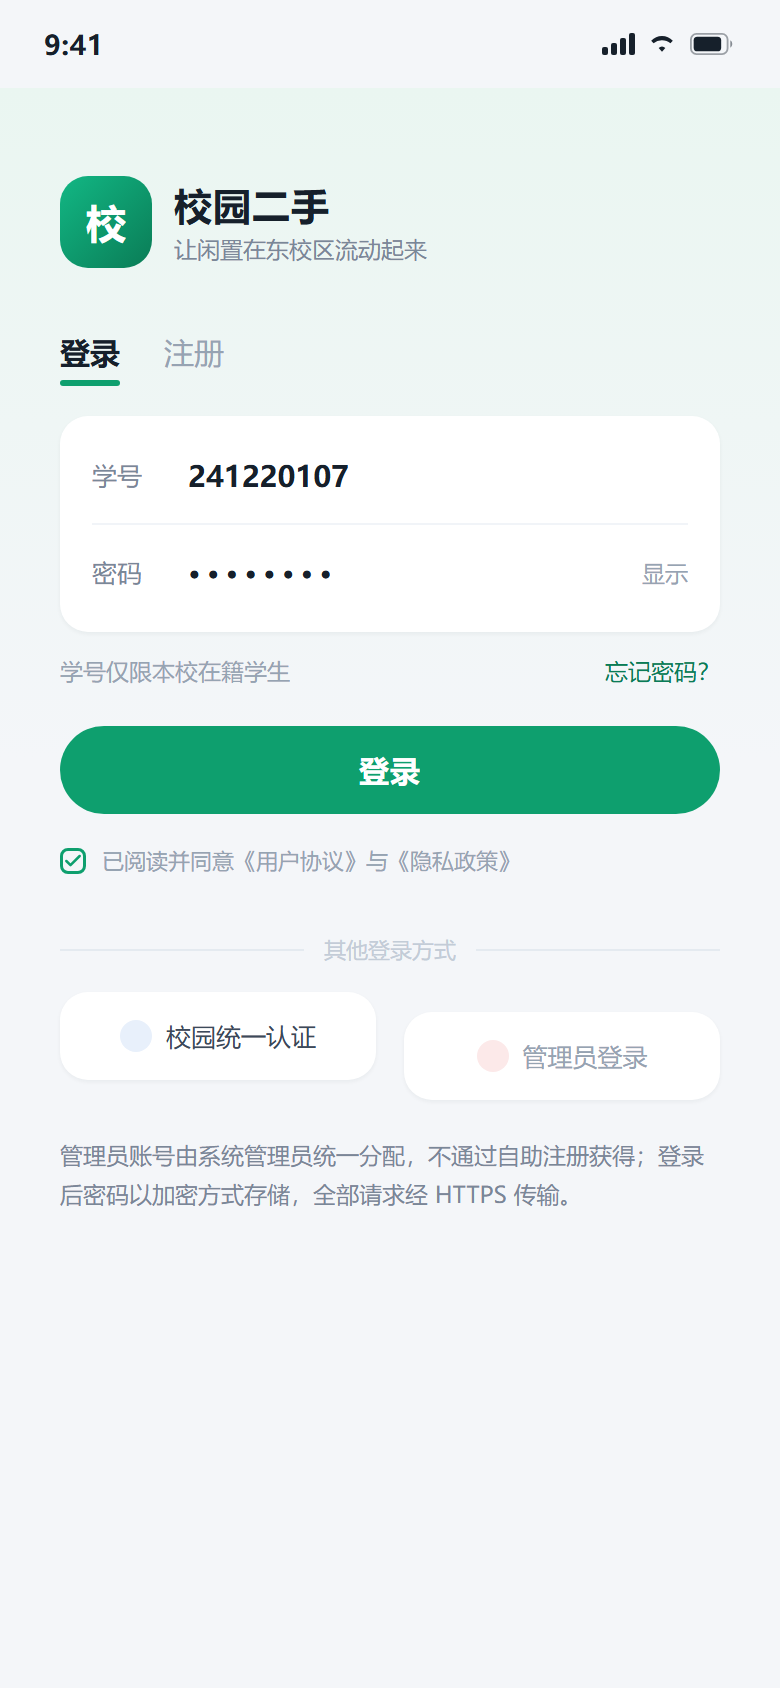
\includegraphics[width=\linewidth]{ui6.png}\end{minipage}
\par\vspace{2pt}
\captionof{figure}{界面 5 我的交易（左）与界面 6 登录 / 注册（右）}\label{fig:ui56}
\end{minipage}
\end{center}

\textbf{界面 5}：分“我买到的”与“我卖出的”两个视角，本图为卖家视角。每张卡片包含状态条、商品信息、四段式进度条（预约—确认—交付—完成）、提示条与操作按钮。进度条让用户一眼看出卡在哪一步；提示条写明“确认后请在 7 天内完成交付，超时系统将自动标记完成”，让 REQ-015 的自动行为可预期，买家视角在同一位置显示倒计时。

\textbf{界面 6}：品牌区、登录/注册切换、学号与密码、协议勾选、其他登录方式。账号字段直接写“学号”并注明“仅限本校在籍学生”，从入口避免重复账号；管理员登录单独作为入口并注明由系统统一分配，对应 REQ-004；页面底部说明密码加密存储与全站 HTTPS，把 REQ-012 的安全约定告知用户。

\subsection{管理后台界面}

\begin{center}
\begin{minipage}{0.80\textwidth}\centering
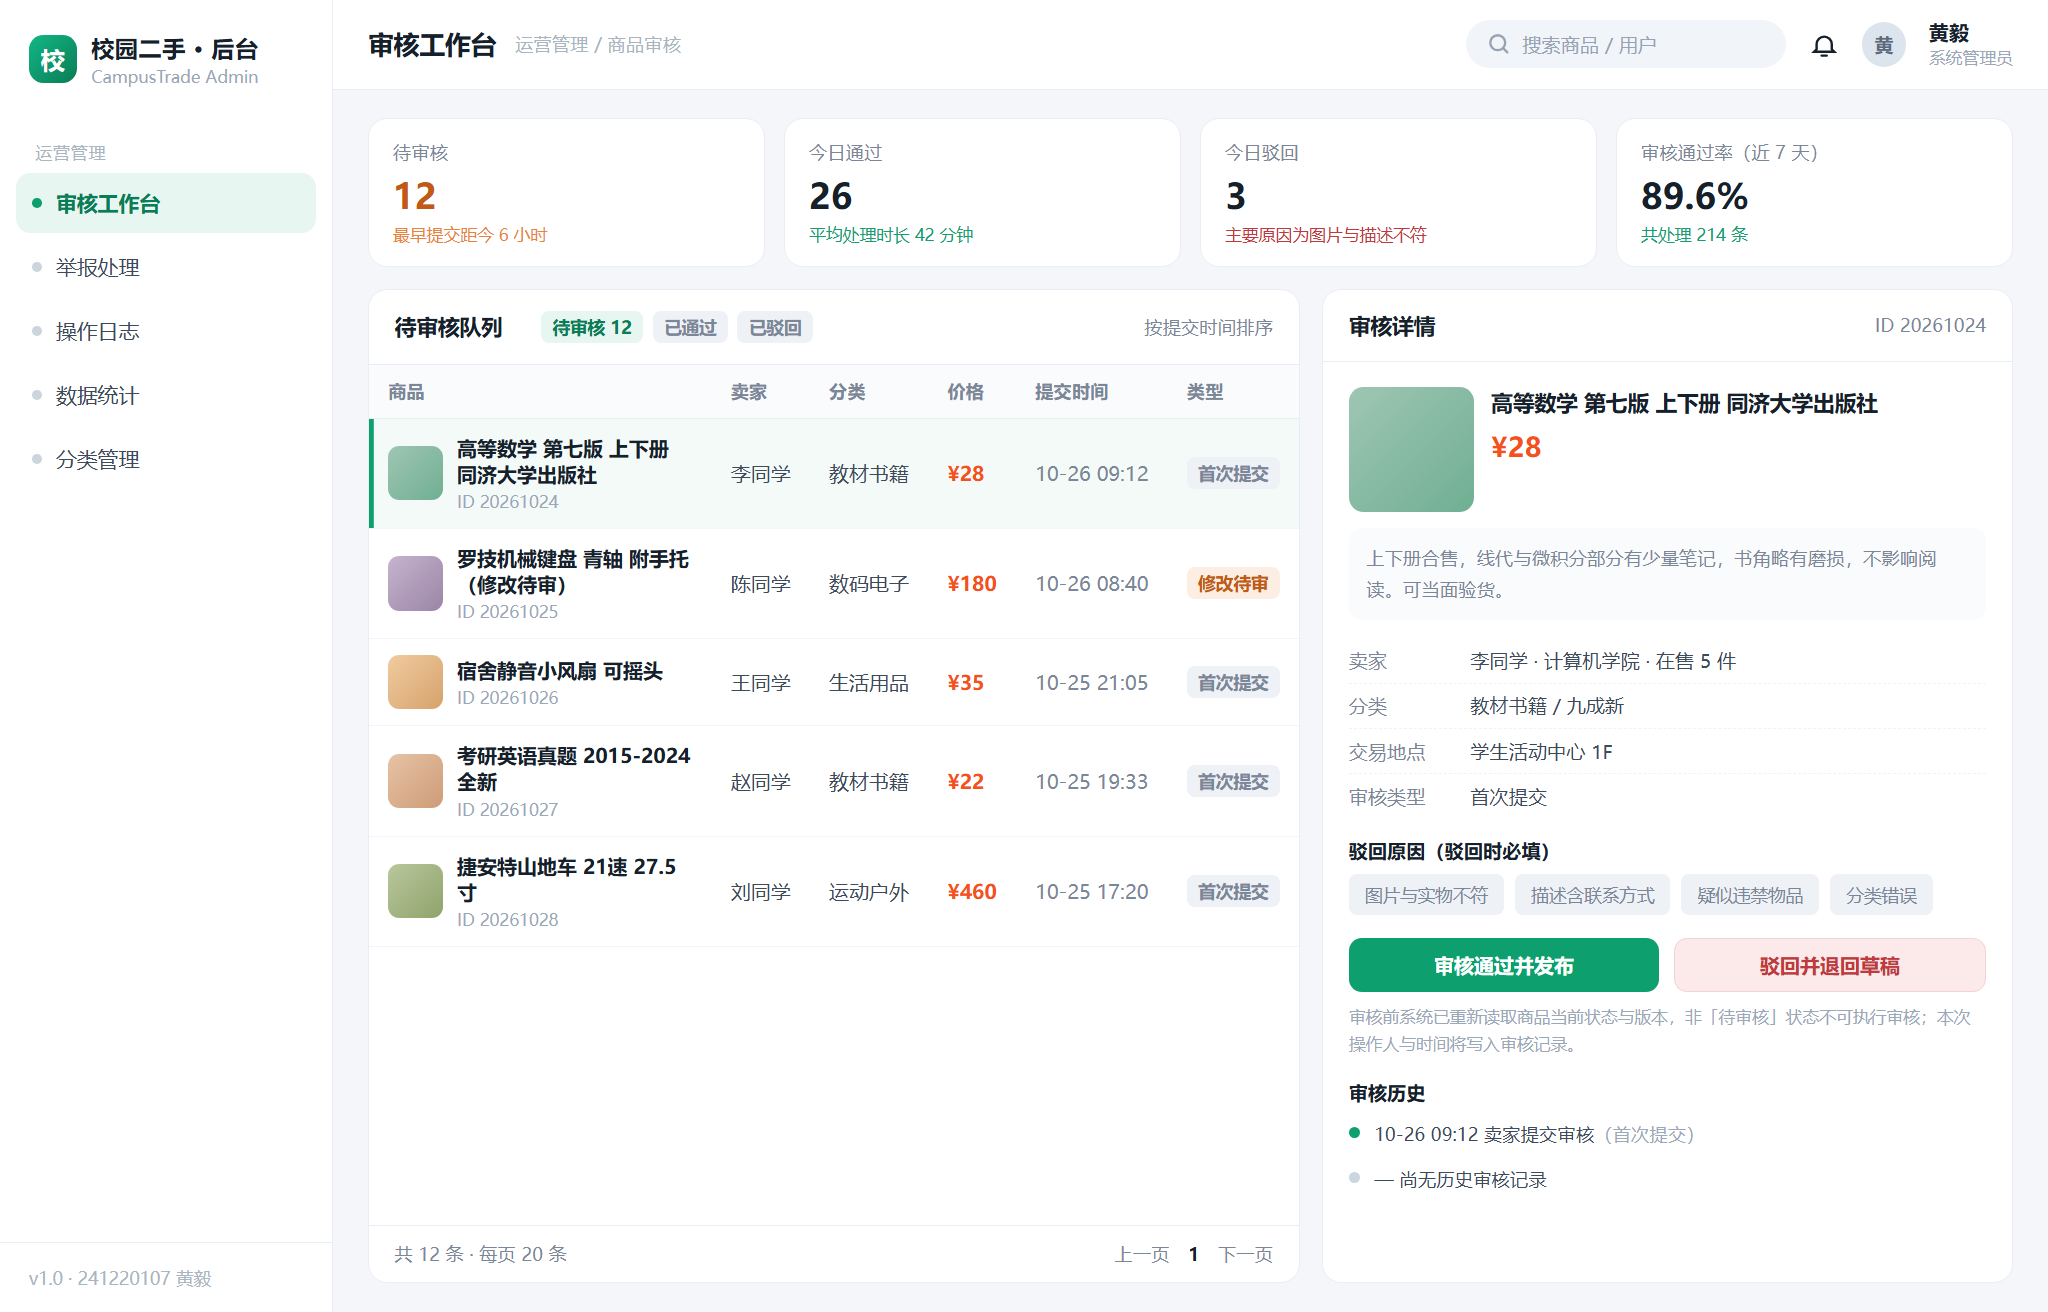
\includegraphics[width=\linewidth]{ui7.png}
\par\vspace{2pt}
\captionof{figure}{界面 7 审核工作台}\label{fig:ui7}
\end{minipage}
\end{center}

顶部指标卡与左侧待审核队列配合使用；驳回原因做成可点选标签而非自由输入，保证原因可统计；按钮下方注明“审核前已重新读取商品状态与版本”，把 REQ-003 的并发处理写在界面上；底部固定展示审核历史，首次提交也显示“尚无记录”。

\begin{center}
\begin{minipage}{0.80\textwidth}\centering
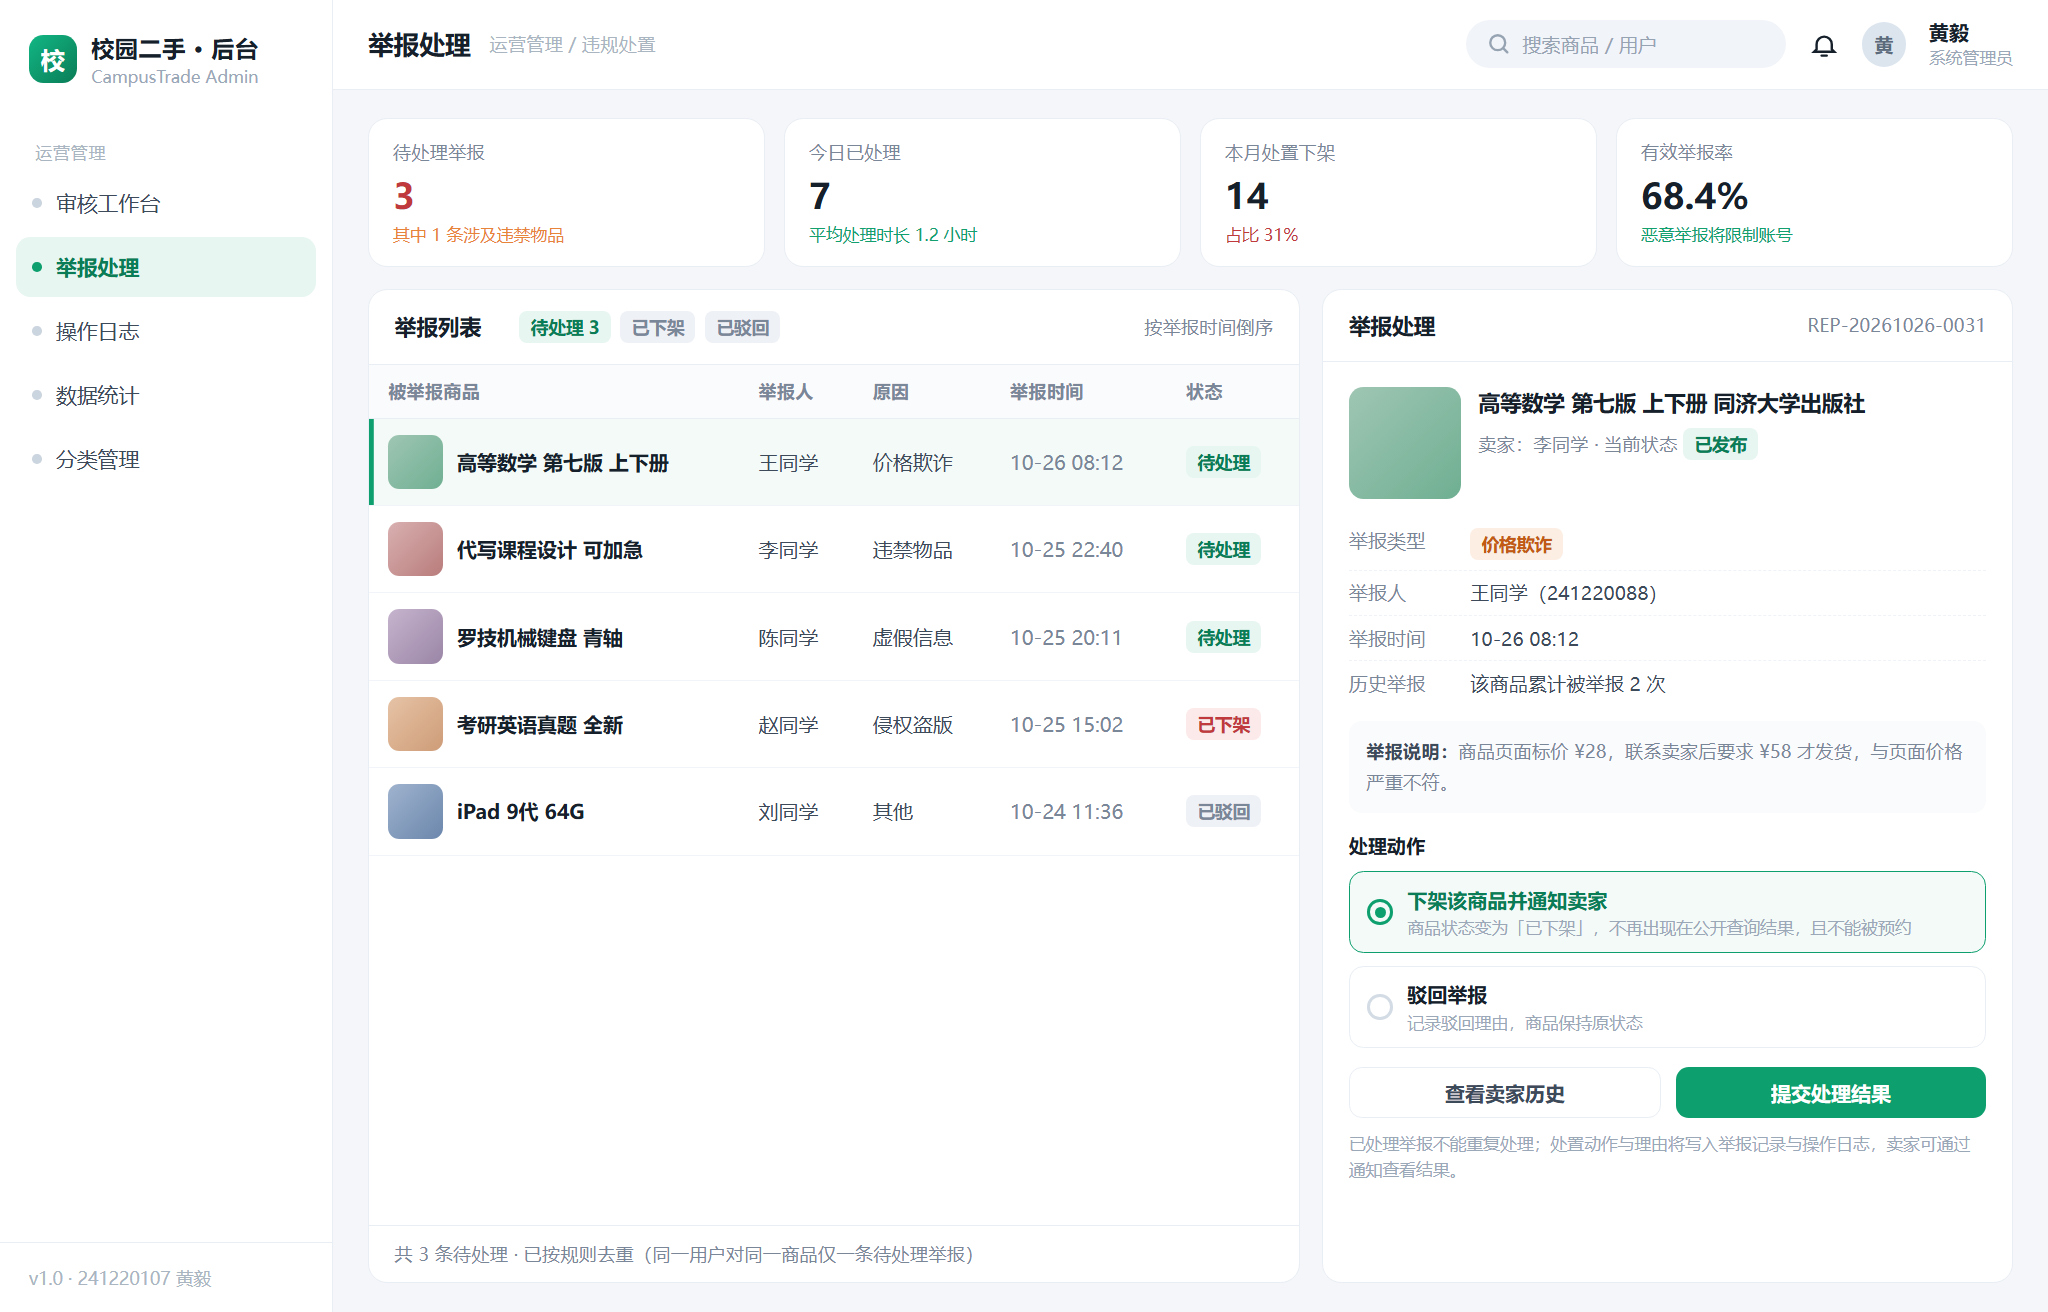
\includegraphics[width=\linewidth]{ui8.png}
\par\vspace{2pt}
\captionof{figure}{界面 8 举报处理}\label{fig:ui8}
\end{minipage}
\end{center}

结构与审核工作台一致。处置动作以单选卡片呈现并展开说明后果（“商品变为已下架，不再出现在查询结果，且不能被预约”），避免不清楚影响就点下架；面板显示累计被举报次数，为判断恶意卖家提供依据。

\begin{center}
\begin{minipage}{0.80\textwidth}\centering
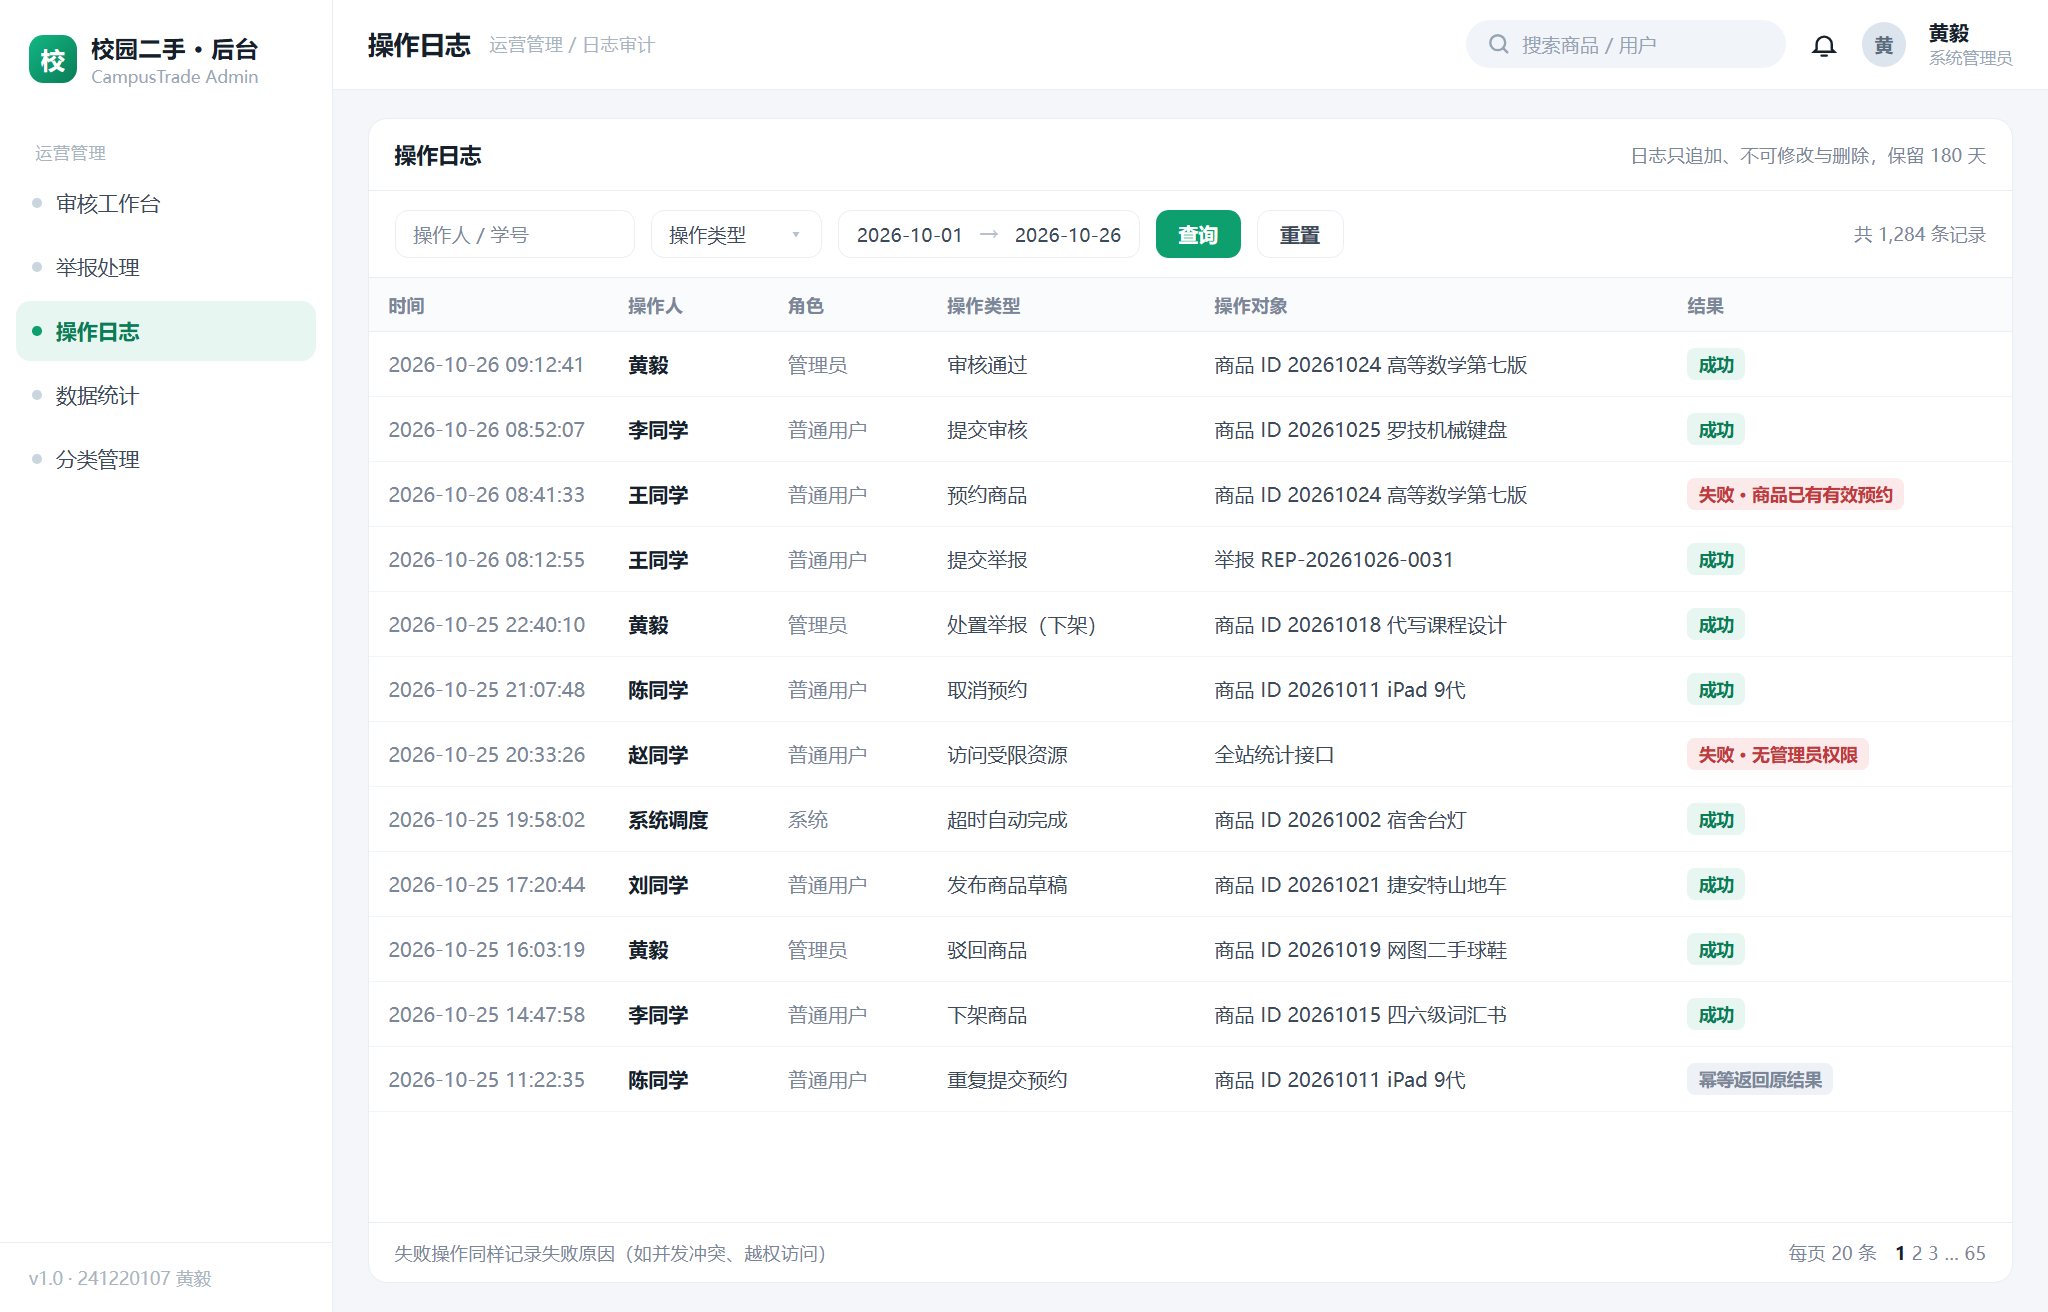
\includegraphics[width=\linewidth]{ui9.png}
\par\vspace{2pt}
\captionof{figure}{界面 9 操作日志查询}\label{fig:ui9}
\end{minipage}
\end{center}

顶部为查询条件（操作人、类型、时间范围），中间为日志表格。结果列含成功与失败，失败项用红色标签写明原因（“失败·商品已有有效预约”“失败·无权限”），对应 REQ-013 的“失败也记录”；顶部标注“只追加、不可修改与删除”。

\begin{center}
\begin{minipage}{0.80\textwidth}\centering
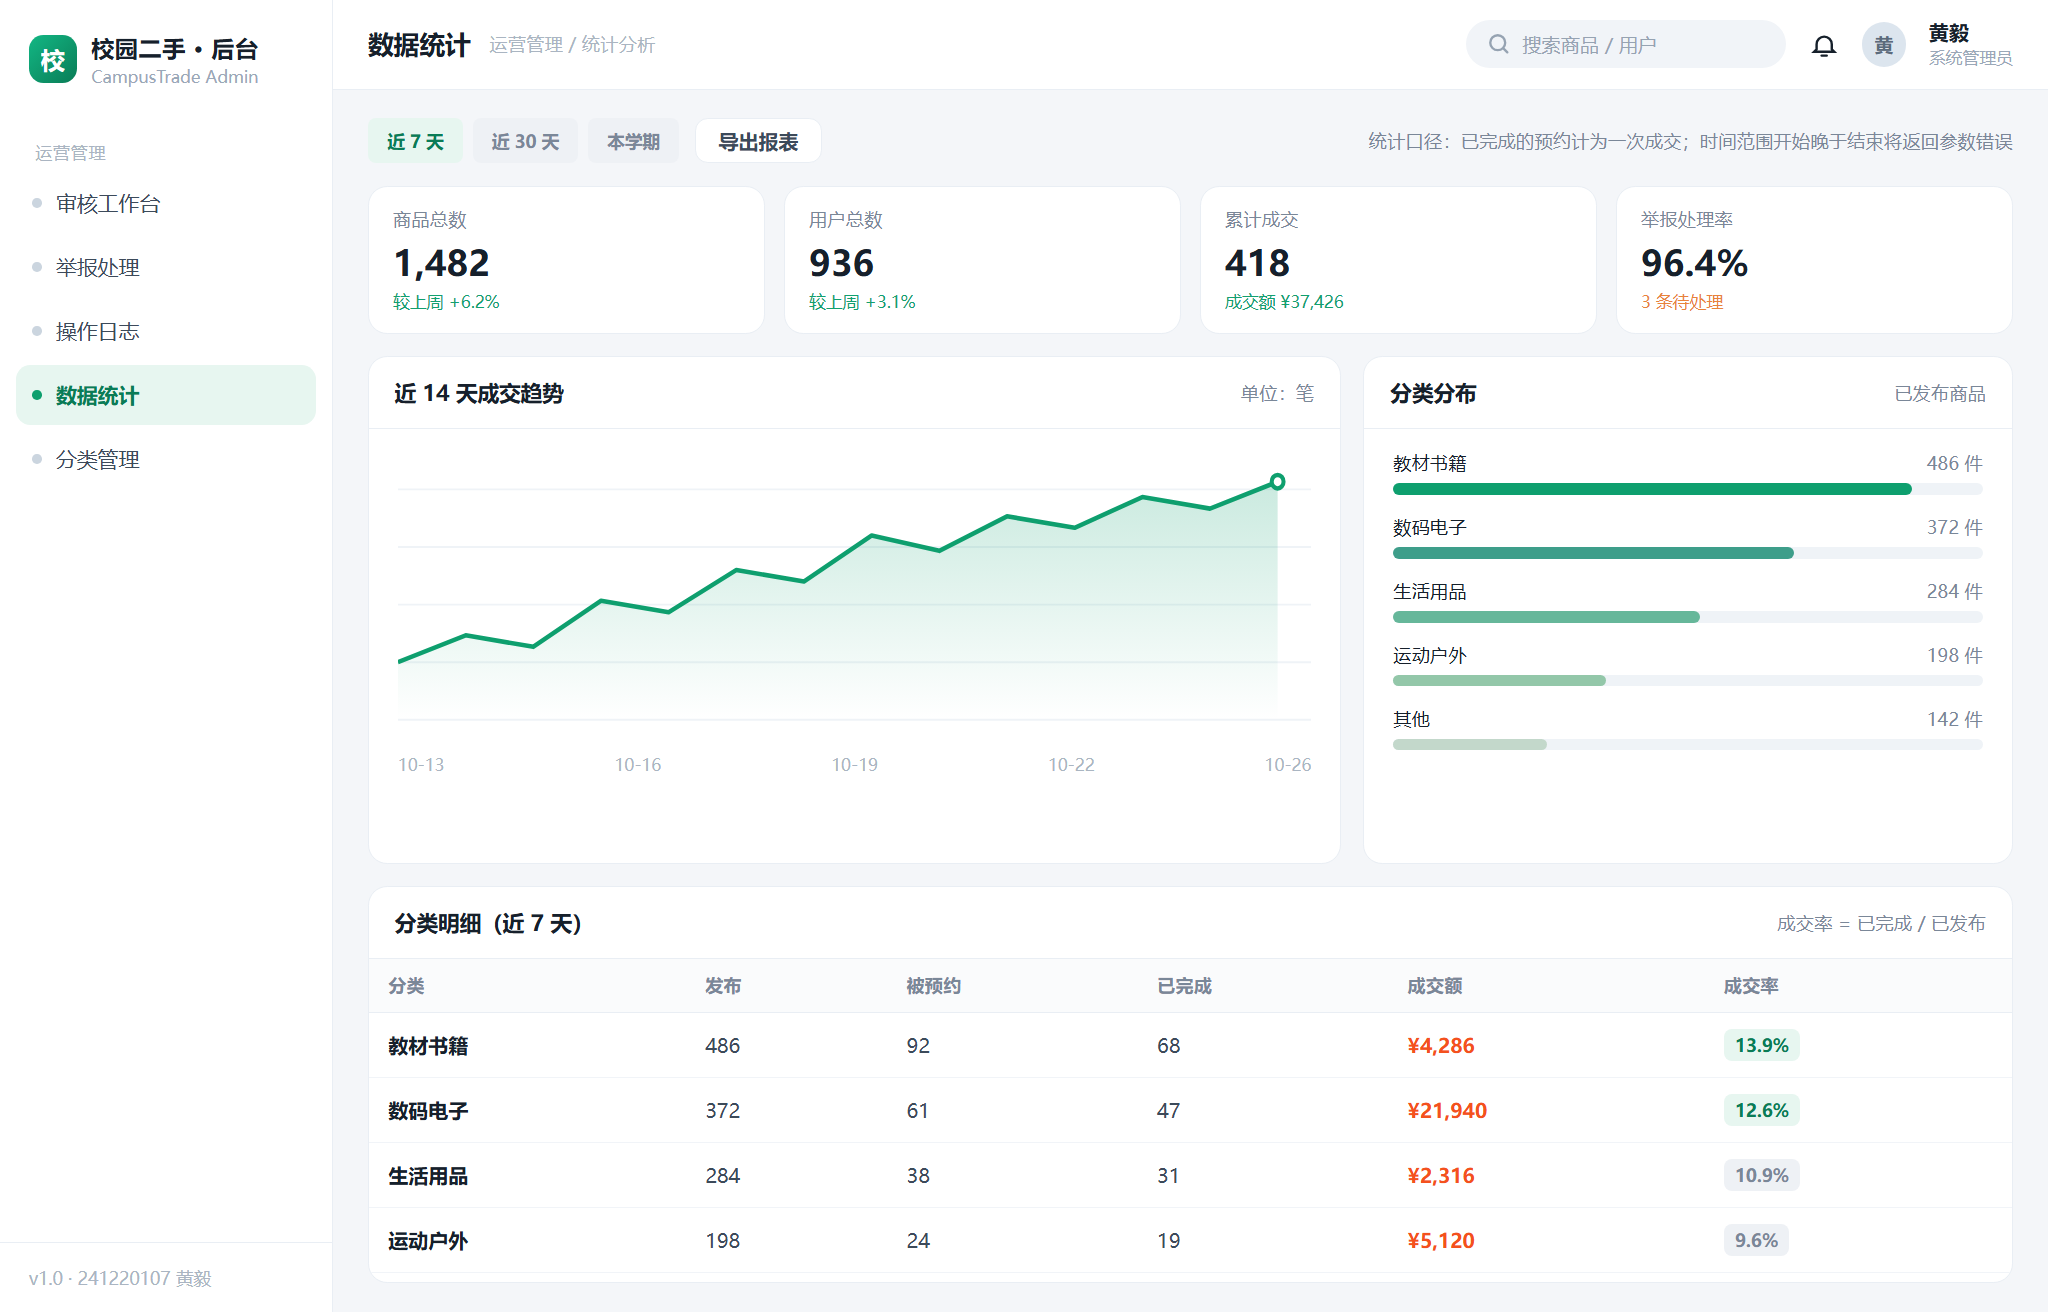
\includegraphics[width=\linewidth]{ui10.png}
\par\vspace{2pt}
\captionof{figure}{界面 10 数据统计}\label{fig:ui10}
\end{minipage}
\end{center}

时间范围切换与导出、四个指标卡、成交趋势、分类分布与明细表。顶部写明口径“已完成的预约计为一次成交”，并提示“时间范围开始晚于结束将返回参数错误”（REQ-018）；卖家视角复用同一页面，范围换成本人。

\clearpage
\section{辅助工具的使用}

本次实验用豆包与 Kimi 参与设计：需求到模块的切分、六类 UML 的样例代码、界面版式与控件方案。三条使用原则：先有自己的判断再问模型（把它当能立刻反驳的同伴，而不是答案来源）；只信可验证的中间产物（能渲染的代码、能逐条核对的表）；输出必须改写进自己的结构，不做“看着不错就贴进去”。

\subsection{使用记录}

五次影响设计的对话见表~\ref{tab:ai}，每次记录场景、生成结果与问题、修改后的结果。

\begin{center}
\captionof{table}{辅助工具使用记录（场景 / 生成结果与问题 / 修改后）}\label{tab:ai}
\zihao{-5}
\renewcommand{\arraystretch}{1.15}
\begin{tabularx}{\textwidth}{@{}p{2.95cm}Yp{5.15cm}@{}}
\toprule
使用场景 & 生成结果与问题 & 修改优化后的结果 \\
\midrule
\textbf{需求到模块}：把 19 条需求与异常清单给它查漏 & 指出“分类管理无模块承接”“定时调度无归属”两处缺口；但 6 模块方案切得过粗，审核要读写商品却独立成模块，也没考虑日志、通知这类横切能力 & 调成 8 模块：分类并入商品，新增日志统计与公共支撑。模型能给覆盖面，给不了“边界切在哪”（表~\ref{tab:module}） \\
\textbf{类图代码}：先列实体清单，让它补属性、方法与多重性 & 24 个类 8 个包，还凭常识加了 Order 实体，与“不保存独立交易事实”冲突；宽高比 4.5:1，放到 A4 上已看不清 & 删 Order；服务类移到组件图；只留 14 个实体与枚举，补组合关系与幂等注释，宽高比降到 1.9:1（\figref{fig:uml1}） \\
\textbf{“修改待审”建模}：把 REQ-017 原文与状态表给它 & 先建议新增“修改待审”状态；追问“驳回后怎么回去”才改为组合状态。代码漏了内部初始转移，且默认“审核期间不能预约”，与需求相反 & 保留组合状态并补三条内部转移；待审内容落成 ItemRevision，驳回即丢弃（\figref{fig:uml5}） \\
\textbf{时序图异常路径}：我写初版，让它检查漏了哪些分支 & 补出“失败也写日志”“通知应在事务提交后发”；但给出“先加锁再查 requestId”，重复请求会排队等锁 & 改为“先查 requestId、未命中再开事务加锁”，三种失败分支全部画进 alt（\figref{fig:uml6}） \\
\textbf{界面布局与控件}：说明“我的商品”要表达状态与动作、后台要排列表与详情 & 三种布局都推荐表格；后台建议左右分栏、驳回原因用下拉框；但 390 宽用表格要横向滚动，下拉框不利于统计，灰阶文字对比度也不足 & 改卡片列表 + 状态标签 + 按状态绑定的按钮；驳回原因改标签组；灰阶文字统一压深（\figref{fig:ui34}） \\
\bottomrule
\end{tabularx}
\end{center}

\subsection{把 AI 放进工作流}

上表的共同点是：模型擅长的部分都能被机器立刻判真假（puml 能否渲染、表格能否逐条核对、截图能否看清），出错的部分都来自它没有的信息（业务约束、版式习惯）。据此可以把流程重排成“模型生成、机器校验、人只做检查校对”，本实验实际跑的五步见表~\ref{tab:aiflow}。

\begin{center}
\begin{minipage}{\textwidth}\centering
\captionof{table}{“模型生成 + 机器校验 + 人工校对”工作流}\label{tab:aiflow}
\zihao{-5}
\renewcommand{\arraystretch}{1.12}
\begin{tabularx}{\textwidth}{@{}p{1.55cm}Yp{4.3cm}p{2.6cm}@{}}
\toprule
环节 & 模型负责 & 人负责 & 可验证的产物 \\
\midrule
① 定骨架 & 不参与 & 从需求划模块、列图清单、写下每张图要表达的结论 & 模块表、图清单 \\
② 出产物 & 生成 puml / 原型 HTML / 表格骨架 & 给约束与字段，点出不合业务的地方 & 能渲染的代码 \\
③ 机器校验 & 不参与 & 渲染、编译、逐条比对需求编号 & 出图、出 PDF \\
④ 检查校对 & 可按清单自查（仅作提醒） & 三张清单：需求覆盖、图形语义、界面一致 & 修订 diff \\
⑤ 入库 & 不参与 & 分次提交并注明 AI 生成或人工修改 & git log \\
\bottomrule
\end{tabularx}
\end{minipage}
\end{center}

“人只做检查校对”成立需要三个前提。其一，每个产物都有机器可判定的通过标准，本实验中是“puml 能渲染且中文不乱码”“PDF 无溢出且图表编号连续”“19 条需求每条都能指到图、表或界面”；没有通过标准的产物（例如“这个架构好不好”）无法交给模型。其二，需求可编号，覆盖关系才能逐条核对，这也是实验一把需求编到 REQ-019 的直接收益。其三，有回退手段，模型整段重写是常事，分次提交后只需撤掉某一次（第~\ref{sec:git} 节）。

剩下唯一不能外包的是检查本身。本报告的文字也用了模型扩写，做法是先自己写下一节的一句话结论与三条要点，再让模型扩成段落，最后拿结论去核对图、截图与需求编号；模型自行添加的判断一律回到产物里验证，验证不了就删。这一轮删掉三处读起来合理但没有依据的句子，例如初稿曾写“审核期间用户不能预约”，与 REQ-017 恰好相反。

\subsection{优缺点与小结}

优点是查漏快、语法模板可靠、概念映射有新角度（把业务描述映射成 UML 组合状态）、方案对比高效。不足是会凭常识造需求、不懂业务约束（认为审核期间不可预约）、没有版式意识、存在顺序与性能盲区（把加锁放在幂等查重之前）、视觉细节不可靠。

由此得到三点判断。其一，这类工具适合做“陪练”而不是“代笔”：设计的核心判断依赖对需求的熟悉程度，模型没有这个上下文，但当先有判断时它能立刻给出反驳与替代方案。其二，它擅长形式、不擅长约束：PlantUML 语法与布局模板表现很好，而“不做支付所以不该有订单”“审核期间仍可预约”这类约束只能来自需求文档。其三，要让输出可被证伪：能立刻渲染的图、能逐条核对的表价值最高。为了让模型理解“修改待审”，我被迫把 REQ-017 逐字读了三遍，才发现自己原以为“审核期间不能预约”——写清问题的过程本身就是一次需求复核。

\clearpage
\section{版本管理与修改追踪}\label{sec:git}

实验二沿用实验一的仓库（\texttt{github.com/APY-tech/Software-Engineering}），不新开仓库。理由有两个：需求与设计同源，回改需求时的 diff 和图形改动留在同一处才能互相对照；按时间回看也能看出“需求 \(\rightarrow\) 设计”的演变，而不是只留一堆最终文件。

提交按“一类产物一次提交、AI 生成与人工修改分开记”拆分，提交说明里写明哪些由模型生成、哪些是人工改的。实验二的主要提交见表~\ref{tab:commit}。

\begin{center}
\captionof{table}{实验二的主要提交与人工改动}\label{tab:commit}
\zihao{-5}
\renewcommand{\arraystretch}{1.15}
\begin{tabularx}{\textwidth}{@{}p{4.65cm}Yp{5.1cm}@{}}
\toprule
提交说明 & 内容 & 类型与人工改动 \\
\midrule
实验二 UML：六图源码与渲染图 & \texttt{UML/*.puml}、\texttt{*.png} & AI 生成初稿；人工修订 7 处（删 Order 实体、服务类移出、改组合状态、幂等前移等） \\
实验二 UI：10 个界面与原型源文件 & \texttt{UI界面/*.png}、\texttt{src/ui} & AI 出版式；人工改列表形态、驳回原因控件、配色令牌 \\
回改实验一：REQ-017 / 001 / 009 & \texttt{requirements.md} v1.1 & 纯人工修改，文末附三条改动理由 \\
实验二 报告 & \texttt{src/report}、实验报告 PDF & 人工写结论与结构；模型辅助扩写，逐条核对后删改 \\
\bottomrule
\end{tabularx}
\end{center}

\textbf{回改实验一的一处实例。}画状态图时发现实验一 REQ-017 写着“修改审核被驳回，商品回到草稿状态”，但同一条又写着“修改审核期间买家仍可预约”——已被预约的已发布商品退回草稿，草稿就带上了有效预约，与“已预约不能修改”也冲突。处理顺序是先改需求（版本升到 v1.1，驳回改为维持已发布、丢弃待审内容），再改图（状态图中“驳回丢弃新内容”的内部转移），两次改动分属两个提交，diff 可以互相对照。若只改图不改需求，实验三按旧需求实现就会写出错误逻辑，这也是回改必须入库、不能只在对话里说一句的原因。

\textbf{为什么分次提交。}模型整段重写很常见，分次提交后只需回退某一次；提交说明标注类型后，review 时可以先看人工修改的 diff（这些才含判断），AI 生成的部分只看是否被完整改写。实验一的提交（AI 初稿 \(\rightarrow\) 人工修正 19 条 \(\rightarrow\) 补 PDF）与实验二沿用同一套习惯：\texttt{git log} 里能区分哪一步是生成、哪一步是判断。

\begin{center}
\captionof{table}{仓库结构与各目录的用途}\label{tab:repo}
\zihao{-5}
\renewcommand{\arraystretch}{1.15}
\begin{tabularx}{\textwidth}{@{}p{4.3cm}Y@{}}
\toprule
路径 & 内容 \\
\midrule
\texttt{实验2\_241220107\_黄毅/} & 交付物：报告 PDF、UML 源码与图、UI 界面图，与提交给课程平台的 zip 内容一致 \\
\texttt{src/ui/} & 界面原型的 HTML/CSS 与导出脚本，10 张界面图由此生成 \\
\texttt{src/report/} & 报告的 LaTeX 源与插图，本 PDF 由此编译 \\
\texttt{requirements.md} & 实验一需求文档，已升至 v1.1 并附回改记录 \\
\bottomrule
\end{tabularx}
\end{center}


\end{document}
